%  A simple AAU report template.
%  2015-05-08 v. 1.2.0
%  Copyright 2010-2015 by Jesper Kjær Nielsen <jkn@es.aau.dk>
%
%  This is free software: you can redistribute it and/or modify
%  it under the terms of the GNU General Public License as published by
%  the Free Software Foundation, either version 3 of the License, or
%  (at your option) any later version.
%
%  This is distributed in the hope that it will be useful,
%  but WITHOUT ANY WARRANTY; without even the implied warranty of
%  MERCHANTABILITY or FITNESS FOR A PARTICULAR PURPOSE.  See the
%  GNU General Public License for more details.
%
%  You can find the GNU General Public License at <http://www.gnu.org/licenses/>.
%
%  A simple AAU report template.
%  2015-05-08 v. 1.2.0
%  Copyright 2010-2015 by Jesper Kjær Nielsen <jkn@es.aau.dk>
%
%  This is free software: you can redistribute it and/or modify
%  it under the terms of the GNU General Public License as published by
%  the Free Software Foundation, either version 3 of the License, or
%  (at your option) any later version.
%
%  This is distributed in the hope that it will be useful,
%  but WITHOUT ANY WARRANTY; without even the implied warranty of
%  MERCHANTABILITY or FITNESS FOR A PARTICULAR PURPOSE.  See the
%  GNU General Public License for more details.
%
%  You can find the GNU General Public License at <http://www.gnu.org/licenses/>.
%
\documentclass[11pt,twoside,a4paper,openright]{report}
%%%%%%%%%%%%%%%%%%%%%%%%%%%%%%%%%%%%%%%%%%%%%%%%
% Language, Encoding and Fonts
% http://en.wikibooks.org/wiki/LaTeX/Internationalization
%%%%%%%%%%%%%%%%%%%%%%%%%%%%%%%%%%%%%%%%%%%%%%%%
% Select encoding of your inputs. Depends on
% your operating system and its default input
% encoding. Typically, you should use
%   Linux  : utf8 (most modern Linux distributions)
%            latin1
%   Windows: ansinew
%            latin1 (works in most cases)
%   Mac    : applemac
% Notice that you can manually change the input
% encoding of your files by selecting "save as"
% an select the desired input encoding.
\usepackage[utf8]{inputenc}
% Make latex understand and use the typographic
% rules of the language used in the document.
\usepackage{subfig}
\usepackage{capt-of}
\usepackage[danish,english]{babel}
% Use the palatino font
\usepackage[sc]{mathpazo}
\linespread{1.05}         % Palatino needs more leading (space between lines)
% Choose the font encoding
\usepackage[T1]{fontenc}
%%%%%%%%%%%%%%%%%%%%%%%%%%%%%%%%%%%%%%%%%%%%%%%%
% Graphics and Tables
% http://en.wikibooks.org/wiki/LaTeX/Importing_Graphics
% http://en.wikibooks.org/wiki/LaTeX/Tables
% http://en.wikibooks.org/wiki/LaTeX/Colors
%%%%%%%%%%%%%%%%%%%%%%%%%%%%%%%%%%%%%%%%%%%%%%%%
% load a colour package
\usepackage{xcolor}
\definecolor{aaublue}{RGB}{33,26,82}% dark blue
% The standard graphics inclusion package
\usepackage{graphicx}
% Set up how figure and table captions are displayed
\usepackage{caption}
\captionsetup{%
  font=footnotesize,% set font size to footnotesize
  labelfont=bf % bold label (e.g., Figure 3.2) font
}
% Make the standard latex tables look so much better
\usepackage{array,booktabs}
\usepackage{tabularx}
% Enable the use of frames around, e.g., theorems
% The framed package is used in the example environment
\usepackage{framed}

%%%%%%%%%%%%%%%%%%%%%%%%%%%%%%%%%%%%%%%%%%%%%%%%
% Mathematics
% http://en.wikibooks.org/wiki/LaTeX/Mathematics
%%%%%%%%%%%%%%%%%%%%%%%%%%%%%%%%%%%%%%%%%%%%%%%%
% Defines new environments such as equation,
% align and split
\usepackage{amsmath}
% Adds new math symbols
\usepackage{amssymb}
% Use theorems in your document
% The ntheorem package is also used for the example environment
% When using thmmarks, amsmath must be an option as well. Otherwise \eqref doesn't work anymore.
\usepackage[framed,amsmath,thmmarks]{ntheorem}

%%%%%%%%%%%%%%%%%%%%%%%%%%%%%%%%%%%%%%%%%%%%%%%%
% Page Layout
% http://en.wikibooks.org/wiki/LaTeX/Page_Layout
%%%%%%%%%%%%%%%%%%%%%%%%%%%%%%%%%%%%%%%%%%%%%%%%
% Change margins, papersize, etc of the document
\usepackage[
  inner=28mm,% left margin on an odd page
  outer=41mm,% right margin on an odd page
  ]{geometry}
% Modify how \chapter, \section, etc. look
% The titlesec package is very configureable
\usepackage{titlesec}
\titleformat{\chapter}[display]{\normalfont\huge\bfseries}{\chaptertitlename\ \thechapter}{20pt}{\Huge}
\titleformat*{\section}{\normalfont\Large\bfseries}
\titleformat*{\subsection}{\normalfont\large\bfseries}
\titleformat*{\subsubsection}{\normalfont\normalsize\bfseries}
%\titleformat*{\paragraph}{\normalfont\normalsize\bfseries}
%\titleformat*{\subparagraph}{\normalfont\normalsize\bfseries}

% Clear empty pages between chapters
\let\origdoublepage\cleardoublepage
\newcommand{\clearemptydoublepage}{%
  \clearpage
  {\pagestyle{empty}\origdoublepage}%
}
\let\cleardoublepage\clearemptydoublepage

% Change the headers and footers
\usepackage{fancyhdr}
\pagestyle{fancy}
\fancyhf{} %delete everything
\renewcommand{\headrulewidth}{0pt} %remove the horizontal line in the header
\fancyhead[RE]{\small\nouppercase\leftmark} %even page - chapter title
\fancyhead[LO]{\small\nouppercase\rightmark} %uneven page - section title
\fancyhead[LE,RO]{\thepage} %page number on all pages
% Do not stretch the content of a page. Instead,
% insert white space at the bottom of the page
\raggedbottom
% Enable arithmetics with length. Useful when
% typesetting the layout.
\usepackage{calc}

%%%%%%%%%%%%%%%%%%%%%%%%%%%%%%%%%%%%%%%%%%%%%%%%
% Bibliography
% http://en.wikibooks.org/wiki/LaTeX/Bibliography_Management
%%%%%%%%%%%%%%%%%%%%%%%%%%%%%%%%%%%%%%%%%%%%%%%%
\usepackage[backend=bibtex,
  bibencoding=utf8,sorting=none
  ]{biblatex}
\addbibresource{bib/mybib}

\usepackage{csquotes}

%%%%%%%%%%%%%%%%%%%%%%%%%%%%%%%%%%%%%%%%%%%%%%%%
% Our own stuff
%%%%%%%%%%%%%%%%%%%%%%%%%%%%%%%%%%%%%%%%%%%%%%%%
%needed for one table
\usepackage{multirow}
%needed for a different table
\newcolumntype{Y}{>{\centering\arraybackslash}X}

%needed for code listings
\usepackage{listings}
%sets the language globally to C
\lstset{language=C}
%code formating
\usepackage{adjustbox}
\usepackage{float}
%\usepackage[usenames,dvipsnames]{xcolor}

\definecolor{codegreen}{rgb}{0,0.6,0}
\definecolor{codegray}{rgb}{0.5,0.5,0.5}
\definecolor{codepurple}{rgb}{0.58,0,0.82}
\definecolor{backcolour}{rgb}{0.95,0.95,0.92}
\definecolor{keywordblue}{rgb}{0.1,0,1}

\lstdefinestyle{CStyle}{
    backgroundcolor=\color{backcolour},
    commentstyle=\color{codegreen},
    keywordstyle=\color{keywordblue},
    numberstyle=\tiny\color{codegray},
    stringstyle=\color{codepurple},
    basicstyle={\footnotesize\ttfamily},
    breakatwhitespace=true,
    breaklines=true,
    captionpos=t,
    keepspaces=true,
    numbers=left,
    numbersep=5pt,
    showspaces=false,
    showstringspaces=false,
    showtabs=false,
    tabsize=2,
    language=C
}
\lstset{style=CStyle}

%%%%%%%%%%%%%%%%%%%%%%%%%%%%%%%%%%%%%%%%%%%%%%%%
% Misc
%%%%%%%%%%%%%%%%%%%%%%%%%%%%%%%%%%%%%%%%%%%%%%%%
% Add bibliography and index to the table of
% contents
\usepackage[nottoc]{tocbibind}
% Add the command \pageref{LastPage} which refers to the
% page number of the last page
\usepackage{lastpage}
% Add todo notes in the margin of the document
\usepackage[
%  disable, %turn off todonotes
  colorinlistoftodos, %enable a coloured square in the list of todos
  textwidth=\marginparwidth, %set the width of the todonotes
  textsize=scriptsize, %size of the text in the todonotes
  ]{todonotes}

%%%%%%%%%%%%%%%%%%%%%%%%%%%%%%%%%%%%%%%%%%%%%%%%
% Hyperlinks
% http://en.wikibooks.org/wiki/LaTeX/Hyperlinks
%%%%%%%%%%%%%%%%%%%%%%%%%%%%%%%%%%%%%%%%%%%%%%%%
% Enable hyperlinks and insert info into the pdf
% file. Hypperref should be loaded as one of the
% last packages
\usepackage{hyperref}
\hypersetup{%
	%pdfpagelabels=true,%
	plainpages=false,%
	pdfauthor={Bucur, Busemann, Klein},%
	pdftitle={P3 project},%
	pdfsubject={Pathfinding, as used in Rescuing Robots},%
	bookmarksnumbered=true,%
	hidelinks,		%no boxes aroundlinks and black fontcolor
	colorlinks=false,%
	citecolor=black,%
	filecolor=black,%
	linkcolor=black,% you should probably change this to black before printing
	urlcolor=black,%
	pdfstartview=FitH%
}
%%%%%%%%%%%%%%%%%%%%%%%%%%%%%%%%%%%%%%%%%%%%%%%%%%%%%%%%%%%%%%%%%%%%%%%%%%%%%%%%%%%%%%%%%%%%%%%%
%%%%%%%%%%%%%%%%%	OUR STUFF
\usepackage{nicefrac}
\newcommand*\mean[1]{\overline{#1}}

%%COLORS FOR COLORCODING FILES IN TODOS%%
\definecolor{c00}	{RGB}{200,200,082}%Acronyms \& Nomenclature
\definecolor{c01}	{RGB}{000,200,082}%Introduction
\definecolor{c02}	{RGB}{200,082,000}%Problem Description
\definecolor{c03}	{RGB}{082,100,200}%Problem Definition
\definecolor{c04}	{RGB}{100,050,200}%Development
  \definecolor{c04a}{RGB}{255,020,200} %Conventional Boost Converter
  \definecolor{c04b}{RGB}{010,200,200} %Switched Inductor
  \definecolor{c04c}{RGB}{200,200,200} %Single Switch Quadratic BC
  \definecolor{c04d}{RGB}{200,200,000} %Three Level BC
  \definecolor{c04x}{RGB}{004,229,069} %Cockroft Walton
  \definecolor{c04y}{RGB}{169,220,090} %Multilevel BC
\definecolor{c05}	{RGB}{050,100,150}%Implementation
  \definecolor{c05a}{RGB}{255,220,000} %Component Specifications
  \definecolor{c05b}{RGB}{210,000,200} %Driver
  \definecolor{c05c}{RGB}{200,200,200} %PCB Design
  \definecolor{c05d}{RGB}{000,200,200} %
  \definecolor{c05x}{RGB}{004,029,249} %
  \definecolor{c04y}{RGB}{069,120,250} %
\definecolor{c06}	{RGB}{150,100,150}%Testing
\definecolor{c07}	{RGB}{050,100,050}%Discussion
\definecolor{c08}	{RGB}{150,100,000}%Conclusion
\definecolor{c09}	{RGB}{050,200,050}%Perspective
\usepackage{pdfpages}
% package inclusion and set up of the document
% see, e.g., http://en.wikibooks.org/wiki/LaTeX/Formatting#Hyphenation
% for more information on word hyphenation
\hyphenation{ex-am-ple hy-phen-a-tion short}
\hyphenation{long la-tex}%
%  A simple AAU report template.
%  2015-05-08 v. 1.2.0
%  Copyright 2010-2015 by Jesper Kjær Nielsen <jkn@es.aau.dk>
%
%  This is free software: you can redistribute it and/or modify
%  it under the terms of the GNU General Public License as published by
%  the Free Software Foundation, either version 3 of the License, or
%  (at your option) any later version.
%
%  This is distributed in the hope that it will be useful,
%  but WITHOUT ANY WARRANTY; without even the implied warranty of
%  MERCHANTABILITY or FITNESS FOR A PARTICULAR PURPOSE.  See the
%  GNU General Public License for more details.
%
%  You can find the GNU General Public License at <http://www.gnu.org/licenses/>.
%
%
%
% see, e.g., http://en.wikibooks.org/wiki/LaTeX/Customizing_LaTeX#New_commands
% for more information on how to create macros

%%%%%%%%%%%%%%%%%%%%%%%%%%%%%%%%%%%%%%%%%%%%%%%%
% Macros for the titlepage
%%%%%%%%%%%%%%%%%%%%%%%%%%%%%%%%%%%%%%%%%%%%%%%%
%Creates the aau titlepage
\newcommand{\aautitlepage}[3]{%
  {
    %set up various length
    \ifx\titlepageleftcolumnwidth\undefined
      \newlength{\titlepageleftcolumnwidth}
      \newlength{\titlepagerightcolumnwidth}
    \fi
    \setlength{\titlepageleftcolumnwidth}{0.5\textwidth-\tabcolsep}
    \setlength{\titlepagerightcolumnwidth}{\textwidth-2\tabcolsep-\titlepageleftcolumnwidth}
    %create title page
    \thispagestyle{empty}
    \noindent%
    \begin{tabular}{@{}ll@{}}
      \parbox{\titlepageleftcolumnwidth}{
        \iflanguage{danish}{%
          
\includegraphics[width=\titlepageleftcolumnwidth]{figures/aau_logo_da}
        }{%
          
\includegraphics[width=\titlepageleftcolumnwidth]{figures/aau_logo_en}
        }
      } &
      \parbox{\titlepagerightcolumnwidth}{\raggedleft\sf\small
        #2
      }\bigskip\\
       #1 &
      \parbox[t]{\titlepagerightcolumnwidth}{%
      \textbf{Abstract:}\bigskip\par
        \fbox{\parbox{\titlepagerightcolumnwidth-2\fboxsep-2\fboxrule}{%
          #3
        }}
      }\\
    \end{tabular}
    \vfill
    \iflanguage{danish}{%
      \noindent{\footnotesize\emph{Rapportens indhold er frit tilgængeligt, men offentliggørelse (med kildeangivelse) må kun ske efter aftale med forfatterne.}}
    }{%
      \noindent{\footnotesize\emph{The content of this report is freely available, but publication (with reference) may only be pursued due to agreement with the authors.}}
    }
    \clearpage
  }
}

%Create english project info
\newcommand{\englishprojectinfo}[8]{%
  \parbox[t]{\titlepageleftcolumnwidth}{
    \textbf{Title:}\\ #1\bigskip\par
    \textbf{Theme:}\\ #2\bigskip\par
    \textbf{Project Period:}\\ #3\bigskip\par
    \textbf{Project Group:}\\ #4\bigskip\par
    \textbf{Participant(s):}\\ #5\bigskip\par
    \textbf{Supervisor(s):}\\ #6\bigskip\par
    \textbf{Copies:} #7\bigskip\par
    \textbf{Page Numbers:} \pageref{LastPage}\bigskip\par
    \textbf{Date of Completion:}\\ #8
  }
}

%Create danish project info
\newcommand{\danishprojectinfo}[8]{%
  \parbox[t]{\titlepageleftcolumnwidth}{
    \textbf{Titel:}\\ #1\bigskip\par
    \textbf{Tema:}\\ #2\bigskip\par
    \textbf{Projektperiode:}\\ #3\bigskip\par
    \textbf{Projektgruppe:}\\ #4\bigskip\par
    \textbf{Deltager(e):}\\ #5\bigskip\par
    \textbf{Vejleder(e):}\\ #6\bigskip\par
    \textbf{Oplagstal:} #7\bigskip\par
    \textbf{Sidetal:} \pageref{LastPage}\bigskip\par
    \textbf{Afleveringsdato:}\\ #8
  }
}

%%%%%%%%%%%%%%%%%%%%%%%%%%%%%%%%%%%%%%%%%%%%%%%%
% An example environment
%%%%%%%%%%%%%%%%%%%%%%%%%%%%%%%%%%%%%%%%%%%%%%%%
\theoremheaderfont{\normalfont\bfseries}
\theorembodyfont{\normalfont}
\theoremstyle{break}
\def\theoremframecommand{{\color{gray!50}\vrule width 5pt \hspace{5pt}}}
\newshadedtheorem{exa}{Example}[chapter]
\newenvironment{example}[1]{%
		\begin{exa}[#1]
}{%
		\end{exa}
}% my new macros

\begin{document}
%frontmatter
\pagestyle{empty} %disable headers and footers
\pagenumbering{roman} %use roman page numbering in the frontmatter
\newcommand{\HRule}{\rule{\linewidth}{0.5 mm}}
\begin{titlepage}

\begin{center}
% Upper part of the page
\iflanguage{danish}{%
	
\includegraphics[width=0.6\textwidth]{figures/aau_logo_da}
}{%
	
\includegraphics[width=0.6\textwidth]{figures/aau_logo_en}
}\\[0.5cm]

\textsc{\Large P5}\\[0.6cm]

% Title
\HRule \\[0.8cm]
{ \Huge \bfseries  Cool Title}\\[0.4cm]

  \Large{ - and subtitulatsia -
  % insert your subtitle here
  }
\HRule \\[1.2cm]

% Author and supervisor
\begin{minipage}{0.49\textwidth}
\begin{flushleft} \large
\emph{Students:}\\
Daniel Frederik Busemann\\
Ilian Oleg Haralampiev\\
Ivan Petrov Kulin\\
Simon Thies\\
\end{flushleft}
\end{minipage}
\begin{minipage}{0.49\textwidth}
\begin{flushright} \large
\emph{Supervisors:} \\
Sanjeevikumar Padmanaban
\end{flushright}
\end{minipage}

\vfill

% Bottom of the page
{\large \today}



\end{center}

\end{titlepage}

%%  A simple AAU report template.
%  2015-05-08 v. 1.2.0
%  Copyright 2010-2015 by Jesper Kjær Nielsen <jkn@es.aau.dk>
%
%  This is free software: you can redistribute it and/or modify
%  it under the terms of the GNU General Public License as published by
%  the Free Software Foundation, either version 3 of the License, or
%  (at your option) any later version.
%
%  This is distributed in the hope that it will be useful,
%  but WITHOUT ANY WARRANTY; without even the implied warranty of
%  MERCHANTABILITY or FITNESS FOR A PARTICULAR PURPOSE.  See the
%  GNU General Public License for more details.
%
%  You can find the GNU General Public License at <http://www.gnu.org/licenses/>.
%
\pdfbookmark[0]{Front page}{label:frontpage}%
\begin{titlepage}
  \addtolength{\hoffset}{0.5\evensidemargin-0.5\oddsidemargin} %set equal margins on the frontpage - remove this line if you want default margins
  \noindent%
  \begin{tabular}{@{}p{\textwidth}@{}}
    \toprule[2pt]
    \midrule
    \vspace{0.2cm}
    \begin{center}
    \Huge{\textbf{
  	  COOL TITLE% insert your title here
    }}
    \end{center}
    \begin{center}
      \Large{
        - EVEN COOLER SUBTITLE -% insert your subtitle here
      }
    \end{center}
    \vspace{0.2cm}\\
    \midrule
    \toprule[2pt]
  \end{tabular}
  \vspace{4 cm}
  \begin{center}
    {\large
      Project Report%Insert document type (e.g., Project Report)
    }\\
    \vspace{0.2cm}
    {\Large
      ED4-1-F18%Insert your group name or real names here
    }
  \end{center}
  \vfill
  \begin{center}
  Aalborg University\\
  Electronics and Computer Engineering
  \end{center}
\end{titlepage}
\clearpage
\thispagestyle{empty}
{\small
\strut\vfill % push the content to the bottom of the page
\noindent Copyright \copyright{} Aalborg University 2018\par
\vspace{0.2cm}
\noindent \LaTeX \: was used for typesetting this report,
MatLab, Simulink, EAGLE and LTSpice were used for designing and verifying the converter and
GitHub \cite{GitHub} for collaborating as a group.
}
\clearpage
\pdfbookmark[0]{Abstract and Information}{label:titlepage_en}
\aautitlepage{%
  \englishprojectinfo{
    %title 
    Non-inverting Multilevel\\
    DC-DC Boost Converter For\\
    Photovoltaic Applications
  }{%
    Signal Processing%theme
  }{%
    Fall Semester 2018 %project period
  }{%
    ED5-3-F18 % project group %TODO
  }{%
    %list of group members
    Daniel Frederik Busemann\\
    Ilian Oleg Haralampiev\\
    Ivan Petrov Kulin\\
    Simon Thies
  }{%
    %ls
    Sanjeevikumar Padmanaban
  }{%
    1 % number of printed copies
  }{%
    \today % date of completion
  }%
}{%department and address
  \textbf{Electronics and Computer Engineering}\\
  Aalborg University\\
  \href{http://www.aau.dk}{http://www.aau.dk}
}{% the abstract
	This report focuses on developing and testing a suitable DC-DC converter for PV applications.
	
	The main goal is to analyse, simulate and compare different topologies and choose the most efficient one. The chosen topology has been tested in hardware as well, to determine its real world viability and how accurate simulations are compared to real measurements.
	The topology chosen is far superior to the the conventional boost converter, as it has gain 6 times higher on all duty cycles. 
	
	For simulation the tools used are SIMULINK and LTSpice. For the hardware test a custom PCB has been designed and printed with a SKYPER driver board being used to operate the circuit.
	
}
\cleardoublepage
\cleardoublepage
\chapter*{Preface\markboth{Preface}{Preface}}\label{ch:preface}
\addcontentsline{toc}{chapter}{Preface}
This report was made by three students from Aalborg University Esbjerg attending
the 4th semester of the Electronics and Computer Engineering course.
From this point on,
every mention of \textbf{we}, \textbf{the group} or \textbf{the authors} refers to the three co-authors listed below.

All resources produced for this project can be found on the GitHub repository \cite{GitHub}.
Selected resources are also in the appendix.

\vspace{\baselineskip}\hfill Aalborg University, \today
\vfill\noindent

\begin{center}
\begin{minipage}[b]{0.45\textwidth}
 \centering
 \rule{\textwidth}{0.5pt}\\
  Daniel Frederik Busemann\\
 {\footnotesize <dbusem16@student.aau.dk>}
\end{minipage}
\hfill
\begin{minipage}[b]{0.45\textwidth}
 \vspace{20mm}
 \centering
 \rule{\textwidth}{0.5pt}
    Ilian Oleg Haralampiev\\
 {\footnotesize <iharal16@student.aau.dk>}
\end{minipage}
\hfill
%
\begin{minipage}[b]{0.45\textwidth}
 \vspace{20mm}
 \centering
 \rule{\textwidth}{0.5pt}\\
    Ivan Petrov Kulin\\
 {\footnotesize <ikulin16@student.aau.dk>}
\end{minipage}
\hfill
\begin{minipage}[b]{0.45\textwidth}
 \vspace{20mm}
 \centering
 \rule{\textwidth}{0.5pt}
    Simon Thies\\
 {\footnotesize <sthies16@student.aau.dk>}
\end{minipage}
\hfill
\end{center}

%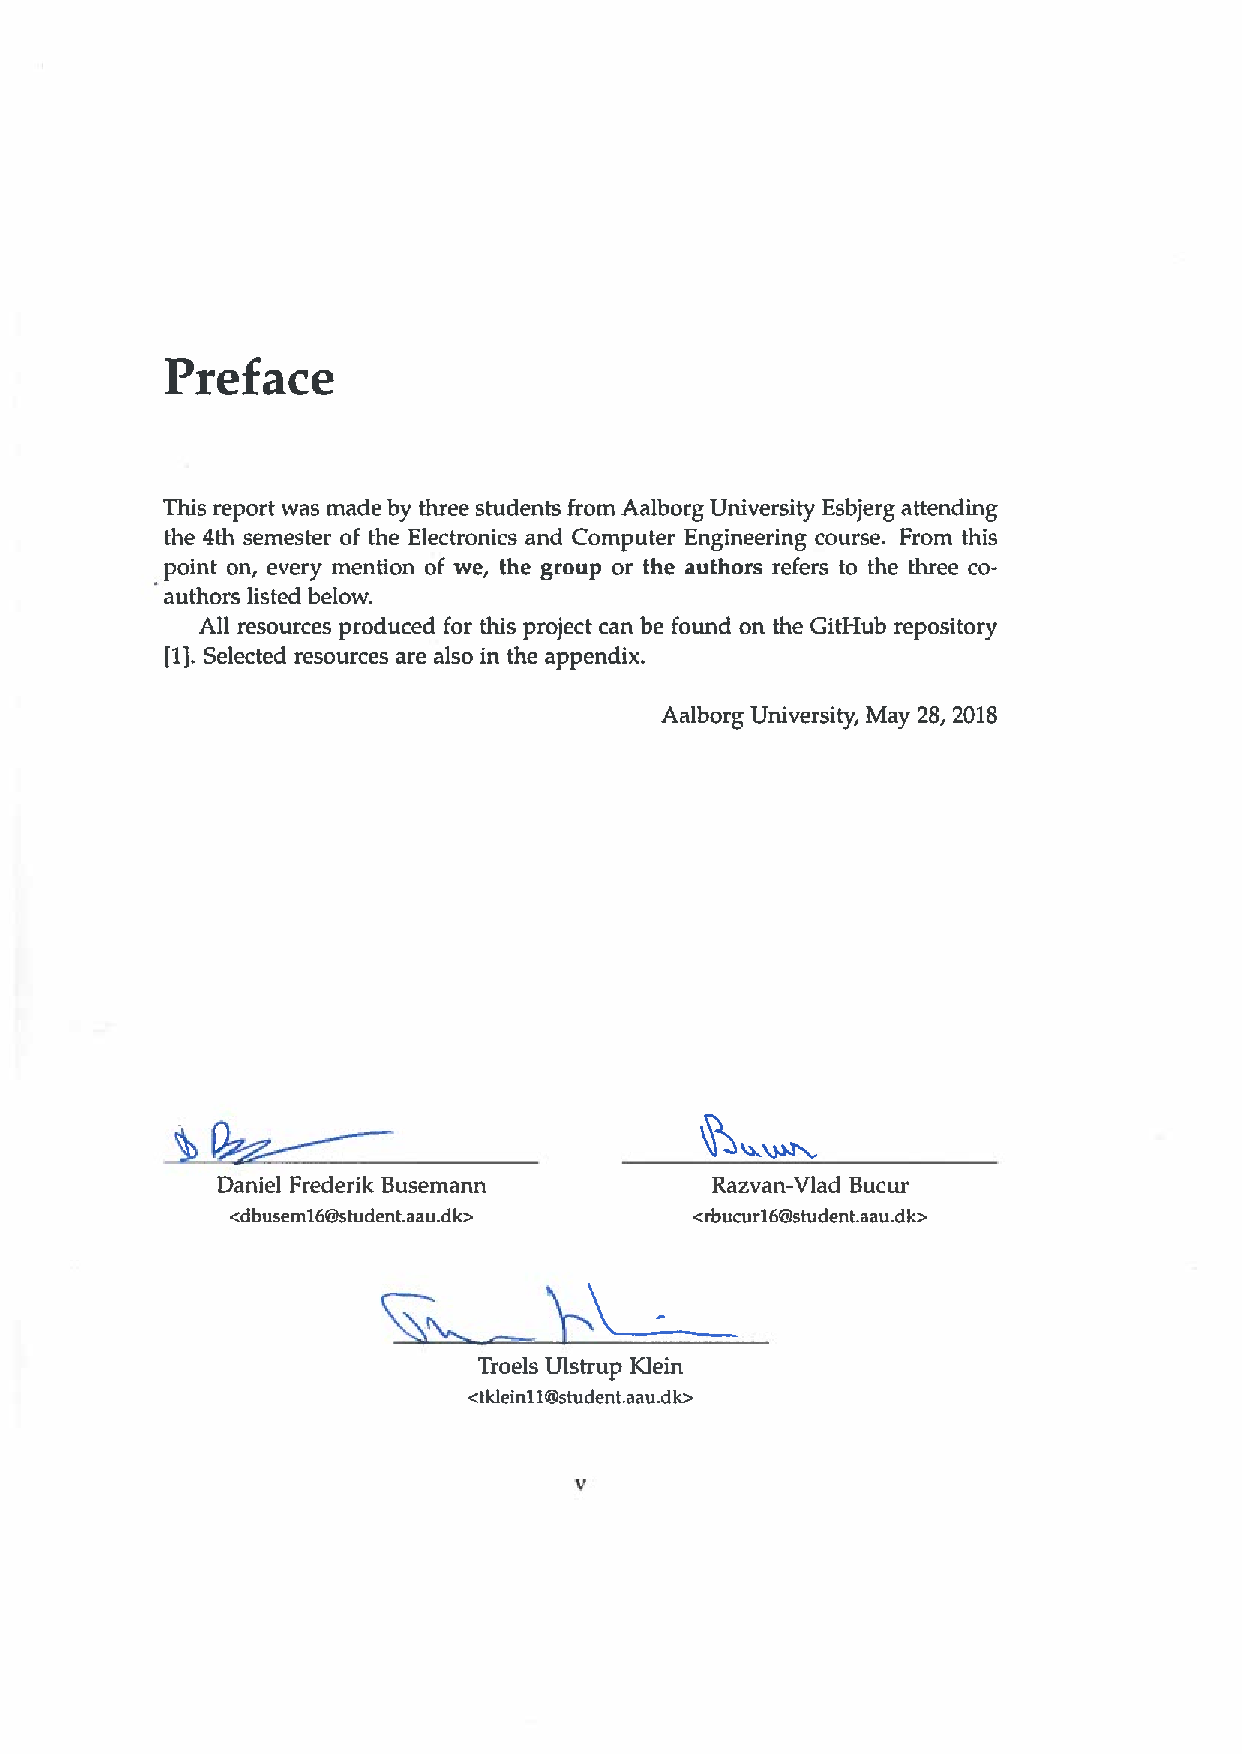
\includepdf[pages=-]{sections/preface.pdf} %TODO this is where the signed page goes
\pdfbookmark[0]{Contents}{label:contents}
\pagestyle{fancy} %enable headers and footers again
\tableofcontents
\listoftodos
\cleardoublepage
%mainmatter
\pagenumbering{arabic} %use arabic page numbering in the mainmatter
\vspace{-24mm}
\section*{Acronyms \& Nomenclature}

\begin{tabular*}{\textwidth}{@{\extracolsep{\fill}} l l r}
	\textbf{Symbol}	& \textbf{Definition}			& \textbf{Unit}\\
	\hline
	AC			& Alternating Current				& \\
	BC			& Boost Converter					& \\
	C			& Capacitance						& $F$\\
	CBC			& Conventional boost converter					& \\
	CTLBC		&Conventional Three Level Boost Converter		& \\
	CWM		    & Cockcroft-Walton Multiplier 		& \\
	DC			& Direct Current					& \\
	D			& Duty cycle					& \\
	f			& Frequency					& $Hz$\\
	I			& Current							& $A$\\
	IVSB		& Inductor Voltage Second Balance				& \\
	KVL			& Kirchhoff's Voltage low				& \\
	L			& Inductance					& $H$\\
	N			& Number of levels						& \\
	P			& Power								& $W$\\
	PV			& Photovoltaic						& \\
	PWM			& Pulse Width Modulation						& \\
	PCB			& Printed Circuit Board					& \\
	R			& Resistance						& $\Omega$\\
	SIBC			&Switched Inductor Boost Converter			& \\
	SISO		& Single Input Single Output		& \\
	SSQBC			&Single Switch Quadratic Boost Converter	& \\
	$T_s$		& Time period					&$s$ \\
	V			& Voltage							& $V$\\
	$\eta$		& Efficiency							&	\\
	\hline \hline
				& \textbf{Subscripts}				&	\\
	\hline
	$ref$		& Reference							&	\\
	$rip$		& Ripple							&	\\
	$tot$		& Total								&	\\
	
	$C$			& Capacitor							&	\\
	$D_i$		& Diode							&	\\
	$L$			& Inductor							&	\\
	$R$			& Resistor							&	\\
	$S$			& Switch							&	\\
	\hline \hline

				& \textbf{Prescripts}				&	\\
	\hline
	$\Delta$	& Change							&	\\
	\hline \hline
\end{tabular*}
\chapter{Introduction}\label{ch:introduction}

As the global interest in renewable energy increases,
the interest in photo voltaic (PV) arrays grows as well. 
Solar power is a growing source of renewable energy on a global scale \cite{solglob}. \todo[color=c01]{ref}
% http://www.ren21.net/wp-content/uploads/2017/06/170607_GSR_2017_Highlights.pdf
This can be indicated by the growing interest power companies show in building PV parks. 
%\cite{solpowcomp}. \todo[color=c01]{find source}

When generating power with PV arrays,
the initial output is a DC power of varying voltage levels. \todo[color=c01]{find source}
To be able to input the generated power into the stable AC-grid,
without creating disturbances,
the same voltage and frequency as the grid needs to be output. \todo[color=c01]{find source}

\begin{figure}[H]
   \centering
   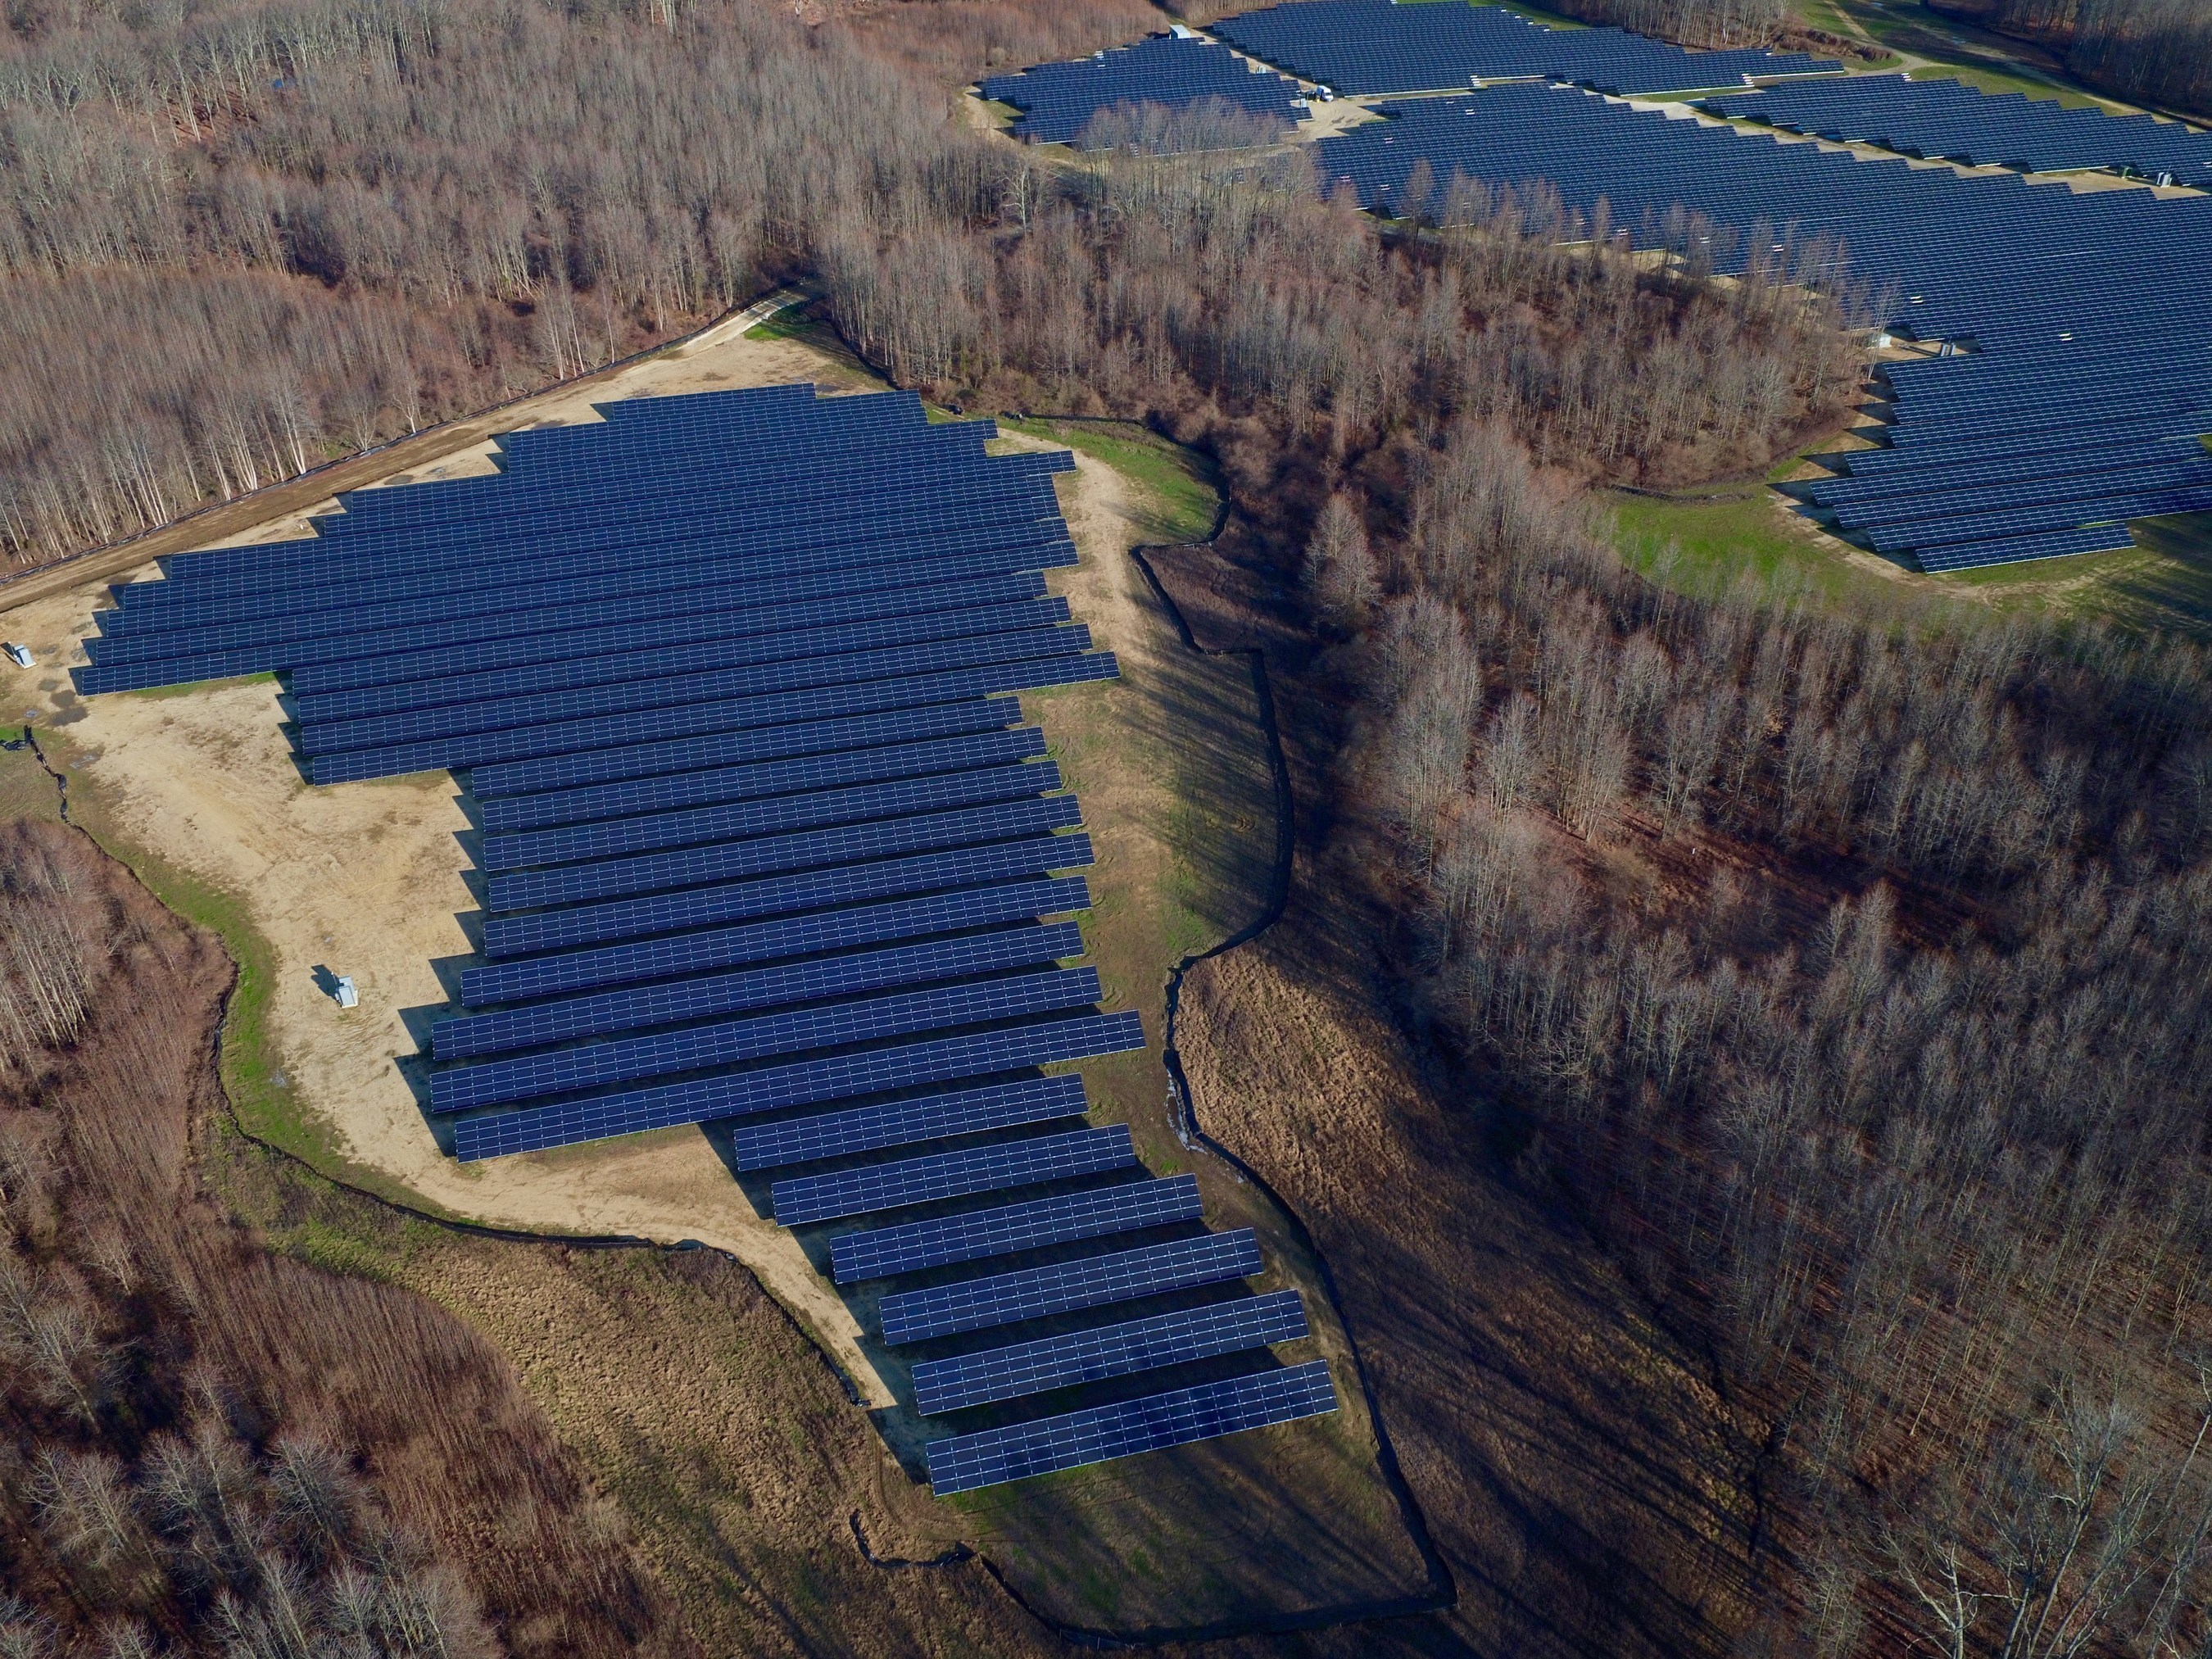
\includegraphics[width=0.8\textwidth]{figures/Problem/solarpark.jpg}
    \caption{12.8 MW Utility Project - the World's Largest Bifacial PV Installation in Eastern US}
	\label{fig:SolarPark}
\end{figure}
\todo[color=c01]{https://www.prnewswire.com/news-releases/sunpreme-deploys-the-worlds-largest-bifacial-pv-installation-for-a-128-mw-utility-project-in-eastern-us-300325989.html}
Commonly this is achieved by two devices,
a DC-DC boost converter (BC) to normalize the voltage
and an DC-AC inverter to generate AC power with the necessary frequency.

In this project we have a look at DC-DC boost converters.
The first part of the project is understanding and simulating common topologies.
The second part is understanding, simulating and building a new topology,
the 2NX Interleaved Boost Converter. \todo[color=c01]{Sanjee's paper is the source}


\section*{Reading Guide}
For readers without an understanding of DC-DC converters,
it is recommended to read the Chapters \ref{ch:basicI}-\ref{ch:basicII}, \todo[color=c01]{ref basic knowledge chapters}
before reading the Chapters \ref{ch:more_advancedI}-\ref{ch:more_advancedII}. \todo[color=c01]{ref advanced chapters}
as these require a deeper understanding.
\chapter{Problem Analysis}\label{ch:probdesc}



\section{Photovoltaic power}
While plants using fossil fuels or nuclear power are outputting high voltage AC directly into the grid, the renewable sources need to be boosted to high voltage, before they can feed their energy into the grid. 
Especially Solar panels produce very low DC-voltage. \cite{PanasonicSolarPanel}
%\todo[color=c01]{ref}
% https://panasonic.net/ecosolutions/solar/product/product_detail/index.html

The setup to supply the energy to the grid can be seen in Figure \ref{fig:SolarConverters}.
There are three stages between converting solar to electric power and inputting that power into the grid. 
First, the low voltage DC coming in from the panel needs to be boosted, before an inverter makes it alternating. Finally  an AC-AC converter 

This three steps involve complicated circuitry, large costs and significant power losses. 
This remains one of the big reasons why solar power is not as cost efficient as other sources that do not require such conversion.

\begin{figure}[H]
   \centering
   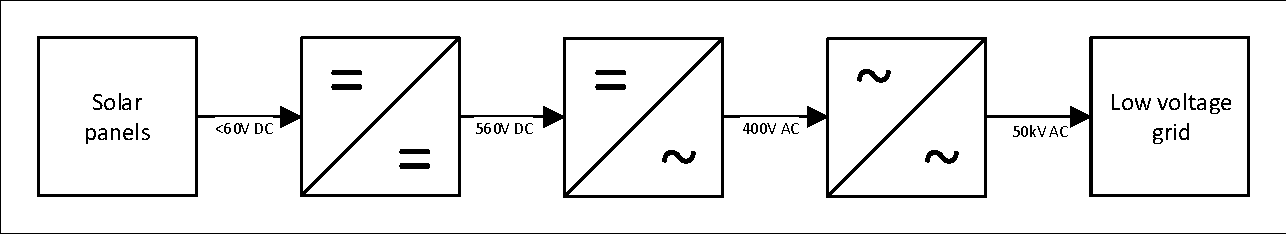
\includegraphics[width=\textwidth]{figures/Problem/SolarConverters.pdf}
    \caption{Connection of solar panels to the grid}
	\label{fig:SolarConverters}
\end{figure}

\section{Problem Description}
This project will focus on trying to improve the first stage or the DC-DC converter. 
The challenge for the boost converter is that the difference is very big.
A typical output of a solar panel is up to 60V DC while the low voltage grid is already 400V AC.
By connecting more panels in series a higher output voltage can be achieved but the power of individual panels can't be used as efficiently.
Using boost converters is the better solution but the standard boost converter topology is not suitable for this case. 
The maximum conversion ratio of the standard converter is limited to a ratio 7.7.
At least cascaded converters are needed to reach the higher internal voltage level.
But they still have to always run on high duty cycles to reach the demanded conversion ratios.
Advanced topologies have higher conversion ratios that may be useful for connecting solar panels.
In general new topologies for boost converters can have advantages over the conventional boost converters when it comes to compactness, efficiency and durability.

 


\chapter{Physical Setup}\label{ch:physsetup}

This chapter explains how the setup is built.
Going into detail about the pump type used,
centrifugal pumps, since they determine the major dynamics of the system.
The other components, pipes, valves and sensors are also explained,
but in less detail.

To give a general overview of the setup,
Figure \ref{fig:setup_photo} shows the front view of the setup,
with all three pumps (red and black) and their individual sensors (blue) visible.
Also visible are the control valve, the target computer,
parts of the electrical wiring and parts of the piping.

\begin{figure}[h]
    \centering
    \includegraphics[width=0.8\textwidth]{photos/setup_photo}
    \caption{Photo of the setup}
    \label{fig:setup_photo}
\end{figure}

Not visible on this photo are the power sensor and the water tank.

A schematic overview of the system is available in Appendix \ref{app:overview}.

This setup was already available for use with student projects
and two other groups used it simultaneously,
which is why no alterations were taken.

\section{Centrifugal Pumps}
A pump is a device used to move liquid through a piping system and to 
raise the pressure of the liquid.
The rise in pressure is often necessary for processes upstream
or to overcome a rise in the pipeline.
We will focus on explaining and describing only centrifugal pumps,
since this is the type of pump present in our setup. 

\subsection{Principle}
In 1689, physicist Denis Papin invented the centrifugal pump. 
It is the most commonly used type of pump, due to its simple construction,
relative low cost, reliability and quiet operation.

The pump is built on a simple principle:
Liquid is led to the impeller hub
and by means of the centrifugal force it is flung towards the periphery of 
the impeller \cite{PumpHandbook}.

Figure \ref{fig:pump_sections} shows two cross sections of a centrifugal pump,
showing the flow of liquid through the pump.
\begin{figure}[h]
    \centering
    \includegraphics[width=0.3\linewidth]{figures/pump_cross_section.PNG}
    \qquad
    \hspace{0.1\textwidth}
    \includegraphics[width=0.3\linewidth]{figures/pump_above_view.PNG}
    \caption{Centrifugal Pump \cite{PumpHandbook}}
    \label{fig:pump_sections}
\end{figure}
\newpage

The fluid is sucked into the impeller at the impeller eye and flows through
the impeller channels formed by the blades between the shroud and hub.
The blades of the rotating impeller transfer energy to the fluid by
increasing velocity and pressure. \cite{CentrifugalPump}

The design of the impeller depends on the requirements for application,
pressure and flow. The impeller is the primary component determining the pump performance. 
Pumps variants are often created only by modifying the impeller.

Changing the impeller size of a pump does not influence all output characteristics equally,
but the change can be modelled with the Affinity Laws.

\subsection{Affinity Laws}\label{sub:afflaws}
Affinity laws are mathematical relationships that provide a way to estimate the 
changes in performance of a pump, as a result of a change in one of the basic pump variables.
In it's simplest form, the term law, means a principle that has been proven true for all cases \cite{Bachus2003}.

Equations \ref{eq:afflaw1} show the relations between a change in motor speeds $N$
to flow $Q$, head $H$ and power $P$.

\begin{equation}
	\frac{Q_1}{Q_2} = \left(\frac{N_1}{N_2}\right)
	\hspace{10mm}
	\frac{H_1}{H_2} = \left(\frac{N_1}{N_2}\right)^2
	\hspace{10mm}
	\frac{P_1}{P_2} = \left(\frac{N_1}{N_2}\right)^3
	\label{eq:afflaw1}
\end{equation}
\cite{Volk2014}\\\\
Similarly, the equations \ref{eq:afflaw2} show the relation between a change in impeller diameter $D$
to  $Q$, $H$ and $P$.

\begin{equation}
	\frac{Q_1}{Q_2} = \left(\frac{D_1}{D_2}\right)
	\hspace{10mm}
	\frac{H_1}{H_2} = \left(\frac{D_1}{D_2}\right)^2
	\hspace{10mm}
	\frac{P_1}{P_2} = \left(\frac{D_1}{D_2}\right)^3
	\label{eq:afflaw2}	
\end{equation}
\cite{Volk2014}

\subsection{Performance Curves}
Performance curves are a very widespread way to compare pumps
and estimate what pump is needed in a specific application.
We included them in this report,
because they also help understanding the relations of $Q$, $H$ and $\omega P$/$N$.

\subsubsection{Pump Head Curve}
A QH-curve or pump curve defines the head as a function of the flow. 
The flow is the rate of the fluid going through the pump.
It is generally stated in cubic meters per hour ($\frac{m^{3}}{h}$).
Figure \ref{fig:typicalPumpCurve} shows a typical pump head curve.
Interesting to notice is,
that the pressure decreases quadratically with the flow.
This can be explained with the Affinity laws mentioned earlier.

\begin{figure}[h]
	\centering
	\includegraphics[width=0.8\textwidth]{figures/03physicalSetup/typicalHeadCurve.PNG}
	\caption{Typical Pump Head Curve \cite{PumpPhoto}}
	\label{fig:typicalPumpCurve}
\end{figure}

\subsubsection{Power Consumption Curve}
The power consumption $P_{el}$ is another key factor,
when choosing a pump for an application.
The typical between $Q$ and $P_{el}$ can be seen in Figure \ref{fig:typicalPowerConsumptionCurve}.
Generally, the power consumption increases with the flow.

\begin{figure}[h]
	\centering
	\includegraphics[width=0.9\textwidth]{figures/03physicalSetup/typicalPowerConsumptionCurve.PNG}
	\caption{Typical Power Consumption Curve \cite{PumpPhoto}}
	\label{fig:typicalPowerConsumptionCurve}
\end{figure}

\subsubsection{Efficiency Curve}
The efficiency $\eta$ of a pump is the relation between the power delivered from the pump to the water $P_{hyd}$ and $P_{el}
$.
Figure \ref{fig:typicalEfficiencyCurve} shows a typical efficiency curve of a pump. The yellow dot represents the 
chosen operating point of the pump. The red dot, shows the efficiency of the pump, at that specific operating point.

\begin{figure}[h]
	\centering
	\includegraphics[width=0.9\textwidth]{figures/03physicalSetup/typicalEfficiencyCurve.PNG}
	\caption{Typical Efficiency Curve (y-axis: H [$ft$]) \cite{PumpPhoto}}
	\label{fig:typicalEfficiencyCurve}
\end{figure}
Noticeable here is,
that $\eta$ does not linearly correlate to $P_{el}$.

\subsubsection{NPSH Curve}
The Net Positive Suction Head (NPSH) is the minimum required pressure
that has to be present at the inlet to avoid cavitation.
The NPSH increases with the flow.
Figure \ref{fig:typicalNPSHCurve} shows a typical NPSH Curve.
It can be observed that for a flow of approximately 32 $gpm$
a NPSH of approximately 8 feet is required.

\begin{figure}[H]
	\centering
	\includegraphics[width=0.9\textwidth]{figures/03physicalSetup/typicalNPSHCurve.PNG}
	\caption{Typical NPSH Curve \cite{PumpPhoto}}
	\label{fig:typicalNPSHCurve}
\end{figure}

\section{Pipes}
Pipes are a way of transporting liquids or gasses, inside a controllable environment.
They are used to interconnect the pumps and the tank and other peripherals.
One common analogy compares them to wires in electrical circuits.

Based on their diameters, material and shape,
they introduce resistance to the flow of the pumped medium.
Staying with the analogy to electrical circuits,
this can be compared to the cross sectional area and the specific resistance of a wire material.

\section{Valves}
A valve is a device used to regulate the flow of a gas or liquid through a piping system.
Valves can be actuated by different means, such as air pressure, electric motors or rotary handles.
The valve present in our setup is a Bürkert control valve.
In our project, we are not using the valve for regulatory purposes,
but only to simulate disturbances and resistance in the system.


\section{Target PC}
A target PC is often used when a setup has to be run in real-time.
In our setup it is a desktop PC running xPC target,
a real-time capable OS.
It is equipped with a PCI card to collect the data from all sensors. \cite{TargetPCSource}
In other cases a different PC setup might be used,
with application specific hardware.
Because the target PC is not a key part of this project,
but merely a tool,
we will not go into detail about it.

\section{Sensors}
When we started the project,
the setup was already equipped with several sensors.
This section will briefly explain what sensors are used.

\subsection*{Flow Meter}
Downstream from  each pump, a magnetic flow meter (MFM) \cite{MFM} is installed to measure the flow.
Their digital gauge was used to calibrate the sensors data output to cubic meters per hour ($\frac{m^3}{h}$).

\subsection*{Power Sensor}
A power sensor \cite{LMG} was used to closely monitor the power delivered to the pumps.
This power works like a digital multimeter,
measuring voltage $U$ and current $I$.
From those measurements it calculates the power $P$.
This sensor has a digital display, where $U$ [$V$], $I$ [$A$] and $P$ [$kW$] are displayed,
which we used to calibrate the output to $kW$.

\subsection*{$\Delta$Pressure Sensor}
Pressure sensors \cite{DPT} are installed across each pump,
measuring the pressure difference between the inlet and the outlet of the pump.
Because they didn't have a visual representation of their measurements
and all our previous calculations of sensor calibration fit with previous work done on the setup \cite{Jepsen2017},
we chose to rely on previous calibration and inherited their conversion.
After this conversion they output data is measured in $bar$.
\chapter{Experiments and Lab Work}\label{ch:experiment}
To relate the theory behind controlling pumps to the real world,
we conducted different experiments.
This helped to gain knowledge about the pump system,
to test controller implementations, and to gather the data needed for tuning of the controller.
\\
All figures shown in this chapter are also available in Appendix \ref{app:gatheredData}.

\section{Data Acquisition}\label{sec:data_gathering}
The pump system is built as described in Chapter \ref{ch:physsetup},
with the controlling PC running xPC Target,
a real-time OS for use with
Simulink\textsuperscript{\textregistered{}} Real-Time\texttrademark{}
(SLRT). 

All data was collected with the help of custom made MATLAB\textsuperscript{\textregistered{}}
(ML) scripts and SLRT models.
The execution of these was done on the xPC Target OS.
Specific parts of these files will be explained in this chapter,
while the complete files can be found on the GitHub repository \cite{GitHub}.

To use SLRT on xPC targets, a SL model of the system was made on the host PC,
compiled, transferred over Ethernet and executed on the xPC target.
After the real-time execution is finished on the target,
the .dat files containing the recorded data have to be transferred back to the host,
where further analysis can be done.

To automate as much of this process as possible,
we created a ML script that updates and compiles the SL model, transfers it to the target,
starts the execution and copies the generated .dat files to the host.

\section{System Test}\label{sec:system_test} 
To obtain information about how the system reacts under different conditions,
a test was carried out with some example conditions.
From those conditions, the goal is to extrapolate an equation for the system,
that can estimate the systems reaction at different conditions.
To obtain the data needed,
a single pump is run at different speeds,
while flow resistance is varied by a choke valve,
resulting in corresponding values of flow, pressure, and energy consumption
measured by the sensors.
The measured data was stored for further analysis such as creating pump curves.

To get an overview over the whole operating range of the setup,
a very broad test was conducted.
We wanted to find the correlations between pump speed, backpressure, flow and power consumption.
To get reliable results, we chose to only change one variable at a time.
Since the value to be changed by our controller was expected to be the pump speed $\omega P_{1,2,3}$,
we decided to fix the backpressure by fixing the control valve position,
and stepwise change $\omega P_{1,2,3}$.
Since the three pumps in the setup are expected to be identical,
the test was only run with one of the pumps.


\subsection{Gathered Data}
Several tests were done on the setup, in order to get a general overview of the system.
Pump 2 was chosen at random.
We have run several tests, where we have gradually changed the pump speed in order to monitor
the flow, pressure and power consumption.
Starting from 0\% pump speed ($\omega P$), we have increased $\omega P$ by 10\% every 15 seconds.
This was done in order to give the system some time to stabilize.
The process was repeated for a range of valve openings.
Similar to $\omega P$, the valve was in the beginning 10\% open,
gradually increasing by 10\% and finally reaching 100\%.
Several identical tests were conducted, in order to see if the values would hold.

Figure \ref{fig:measuredFlow} shows the raw flow measurements,
while Figure \ref{fig:measuredPower} and Figure \ref{fig:measuredPressure} show the
raw power and pressure measurements.
Interesting to notice here is that the lowest values for $Q$ appeared at the lowest values for $CV_1$,
while $P$ behaves in the opposite manner, having its highest values at the lowest $CV_1$.
%\begin{figure}[H]
%	\centering
%	\includegraphics[width=0.8\textwidth]{figures/05mathematicalModelling/measuredFlow.eps}
%	\caption{Measured Flow}
%	\label{fig:measuredFlow}
%\end{figure}
%
%\begin{figure}[H]
%	\centering
%	\includegraphics[width=0.8\textwidth]{figures/05mathematicalModelling/measuredPower.eps}
%	\caption{Measured Power}
%	\label{fig:measuredPower}
%\end{figure}
%
%\begin{figure}[H]
%	\centering
%	\includegraphics[width=0.8\textwidth]{figures/05mathematicalModelling/measuredPressure.eps}
%	\caption{Measured Pressure}
%	\label{fig:measuredPressure}
%\end{figure}

\subsection{Data Example}%\label{sec:results}
To give some more insight in the testing,
we wanted to show the data collected in a single run.
The Figures \ref{fig:measuredFlow}, \ref{fig:measuredPower} and \ref{fig:measuredPressure}
show the collected data through several runs,
each with a different $CV_1$.
The data for all lines $CV_1 = 70\%$ in all three figures comes from the same run.
While executing a run,
the data for all used sensors was shown on the target in real time.
To get a better understanding of how the tests were executed,
we included Figure \ref{fig:testrun},
a rebuilt live view.

%\begin{figure}[H]
%	\centering
%	\includegraphics[width=0.8\textwidth]{figures/04ExperimentsAndLabWork/testrun.eps}
%	\caption{$Q$, $H$, $P$ and stair input $\omega P_{2in}$ at $CV_1 = 70\%$}
%	\label{fig:testrun}
%\end{figure}

\chapter{Mathematical Modelling}\label{ch:mathmodel}

\section{Static Modelling}\label{sec:statmod}

\subsubsection{Single Pump Model}

\begin{equation}
	H = \bar{a_{2}} \cdot Q^2 + \bar{a_{1}} \cdot Q + \bar{a_{0}}
	\label{eq:pumpHeadModel}
\end{equation}
\begin{equation}
	P = \bar{b_{3}} \cdot Q^3 + \bar{b_{2}} \cdot Q^2 + \bar{b_{1}} \cdot Q + \bar{b_{0}}
	\label{eq:pumpPowerModel}
\end{equation}

\begin{align*}
	\left(\frac{\omega_1}{\omega_2}\right)^1 = \frac{Q_1}{Q_2} && 
	\left(\frac{\omega_1}{\omega_2}\right)^2 = \frac{H_1}{H_2} &&
	\left(\frac{\omega_1}{\omega_2}\right)^3 = \frac{P_1}{P_2}		
\end{align*}\cite{Volk2014}.

\begin{equation}
	H(\omega) = a_0 \cdot \omega^2 + a_1 \cdot \omega \cdot Q(\omega) + a_2 \cdot Q(\omega)^2
	\label{eq:pumpHeadModel2}
\end{equation}
\begin{equation}
	P(\omega) = b_0 \cdot \omega^3 + b_1 \cdot \omega^2 \cdot Q(\omega) + b_2 \cdot \omega \cdot Q(\omega)^2 + b_3 \cdot Q(\omega)^3
	\label{eq:pumpPowerModel2}
\end{equation}

\begin{align*}
	a_0 = \frac{\bar{a_0}}{\bar{\omega_0^2}} && a_1 = \frac{\bar{a_1}}{\bar{\omega_0}} && a_2 = \bar{a_2} \\
	b_0 = \frac{\bar{b_0}}{\bar{\omega_0^3}} && b_1 = \frac{\bar{b_1}}{\bar{\omega_0^2}} && b_2 = \frac{\bar{b_2}}{\omega_0} && b_3 = \bar{b_3}
\end{align*}
\cite{Yang2010}

%\begin{figure}[ht]
%	\centering
%	\includegraphics[width=1\textwidth]{figures/05mathematicalModelling/flowVsPowerRun34.eps}
%	\caption{Data Points for Flow vs. Power Consumption}
%	\label{fig:flowVsPowerConsumption}
%\end{figure}

\begin{align*}
	a_0 = -0.03044 && a_1 = 0.07635  && a_2 = 1.688  \\
	b_0 = -0.2825 && b_1 = -0.7147 && b_2 = 54.39 && b_3 = 163.7 \\
\end{align*}

\section{Dynamic Modelling}\label{sec:dynMod}

\begin{equation}
	\frac{Y(s)}{U(s)} = \frac{A \cdot e^{-st_d}}{\tau \cdot s + 1}
	\label{eq:plantTransferFunction}
\end{equation}

\begin{itemize}
	\item A = final value the step response settles at
	\item $t_{d}$ = time delay
	\item $\tau$ = time it takes from 0.1 of final value to 0.9 final value
\end{itemize}

\chapter{Model Validation}\label{ch:modValPerf}
\section{Static Modelling}

\begin{equation}
	H(\omega) = \frac{\bar{a_0}}{\bar{\omega_0^2}} \cdot \omega^2 + \frac{\bar{a_1}}{\bar{\omega_0}} \cdot \omega \cdot Q(\omega) + \bar{a_2} \cdot Q(\omega)^2
	\label{eq:pumpHeadModel60}
\end{equation}
\begin{equation}
	P(\omega) = \frac{\bar{b_0}}{\bar{\omega_0^3}} \cdot \omega^3 + \frac{\bar{b_1}}{\bar{\omega_0^2}} \cdot \omega^2 \cdot Q(\omega) + \frac{\bar{b_2}}{\omega_0} \cdot \omega \cdot Q(\omega)^2 + b_3 \cdot Q(\omega)^3
	\label{eq:pumpPowerModel60}
\end{equation}

\section{Dynamic Modelling}
\chapter{Controller Design}\label{ch:controldesign}
There exist many different approaches to designing a controller,
all of which have their advantages and disadvantages.
For this project we decided to use a very simple approach,
the Proportional Derivative Integral (PID) controller.
This chapter compares this to another possible option,
the state-space controller, explains both of them briefly
and argues for our choice.

\section{PID control}\label{sec:PID}
A PID controller consists of three parts,
a proportional, integral and derivative part,
which it inherits its name from.
A mathematical representation can be given by one of the two equations in Equation \ref{eq:PID}.

\begin{equation}
	  D_{cl}(s) = k_P + \frac{k_I}{s} + k_D s$$
	$$D_{cl}(s) = k_P ( \frac{T_I}{s} + T_D s)
	 \label{eq:PID}
\end{equation} \cite{Franklin2014}\\
These equations can be visualised in block diagrams, as shown in Figure \ref{fig:twoPID}.
\begin{figure}[H]
    \centering
    \includegraphics[width=\textwidth]{figures/07controllerDesign/PID_explicit.pdf}
    \caption{Comparison of two common PID designs}
	\label{fig:twoPID}
\end{figure}

Figure \ref{fig:twoPID} also shows the typical placement of a PID-controller,
on the forward loop, behind the subtraction of the feedback and before the input to the plant.

The gains $k_P$, $k_I$ and $k_D$ have to be tuned according to the dynamics of the plant
and the desired characteristics of the controller.
This tuning can be done manually, or methodically.
We chose to use the Ziegler-Nichols tuning method,
as described by Franklin et al. \cite{Franklin2014},
as this method promised results close to our requirements and was discussed in our courses.

To use this method, some knowledge about the system is required.
If the system reacts stable to a step input,
the output measured can be used to tune $k_P$, $k_I$ and $k_D$
according to the Quarter Decay Method (QDM) \cite{Franklin2014}.

In the case that the system has an unstable reaction,
the Ultimate Sensitivity Method (USM) should be used.
Here the $k_p$ is increased until the system becomes marginally stable.
\cite{Franklin2014}

In both cases the output of the system is to be graphed over time
and from the corresponding graph some characteristic values can be read.
Because we are using the quarter decay method,
we won't discuss the ultimate sensitivity method any further.

As mentioned before,
to use the QDM, we need a step response of the system.
The following section explains step response in more detail and shows our analysis.

\subsection{Quarter Decay Tuning}\label{sub:quadec}
To obtain all needed data, the step response of the system
needs to be analysed.

\subsubsection{Step Response}
The step response needs to be measured on the Open Loop (OL) system.
A block diagram of an OL setup can be seen in Figure \ref{fig:OL}.

\begin{figure}[H]
    \centering
    \includegraphics[width=0.75\textwidth]{figures/07controllerDesign/OLblock.pdf}
    \caption{OL block diagram of a system}
\label{fig:OL}
\end{figure}

The recorded output can be seen in Figure \ref{fig:stepin}.
The figure also shows two red lines, approximating the slope and the final value.

\begin{figure}[H]
    \centering
    \includegraphics[width=\textwidth]{figures/07controllerDesign/StepResponseLabeled.eps}
    \caption{response to a step input with value 10}
	\label{fig:stepin}
\end{figure}

From this graph we can approximate the slope $R$ and the Lag $L=t_d$.\\
Because we are scaling the $\omega P$ down by a factor of 10, so we can directly input a percentage,
we had to scale the aforementioned unit step up by a factor of 10,
in order to get usable results.
While encountering this problem, we also noticed, that the pumps don't spin at $\omega \leq 9\%$.
When using the corrected step input, we got the measurements shown in Figure \ref{fig:stepin}.

Our analysis of figure \ref{fig:stepin} gives us the following values:
\\
\begin{tabular}{r c l l}
	$R$ 	& $=$ & $2.0236$ 	& \footnotesize{\textit{slope}}\\
	$t_d=L$	& $=$ & $0.75$ 		& \footnotesize{\textit{lag}}\\
\end{tabular}


\subsubsection{Tuning}
The QDM is tuning a P, PI or PID controller $D_c(s)$ with the formula shown in the second Equation \ref{eq:PID}.
The values of $k_P$, $T_I$ and $T_D$ are scalar gains,
tuned according to the characteristics obtained from figure \ref{fig:stepin}.
\\
\begin{center}
\begin{tabular}{l r c l l}
	Type of Controller	& \multicolumn{3}{ c }{Optimum Gain}\\
	\hline
	\multirow{1}{*}{P}	& $k_P$ & $=$ & $\nicefrac{1}{RL}$	\\
	\\
	\multirow{2}{*}{PI}	& $k_P$ & $=$ & $\nicefrac{0.9}{RL}$\\
						& $T_I$ & $=$ & $\nicefrac{L}{0.3}$	\\
	\\
	\multirow{3}{*}{PID}& $k_P$ & $=$ & $\nicefrac{1.2}{RL}$\\
						& $T_I$ & $=$ & $2L$				\\
						& $T_D$ & $=$ & $0.5L$ 				\\
\end{tabular}
\end{center}
Note that the parameters $T_I$ and $T_D$ are not mentioned for the first two controller types,
as they are to be set to 0.

\subsubsection{Results}
We tested all three options of P, PI and PID control with the tuned parameters,
the results can be seen in Figure \ref{fig:PIDtest}.
Please note, that the P-controller with the calculated value did not achieve any results,
as the error was too small to start the pump.
To overcome this issue, we multiplied $k_P$ with 10.
This was solely done for the P-controller,
because the PI- and PID-controller gave proper results without this correction.
We expect this to be caused by the scaling factor before the input to the pumps,
as discussed in Subsection \ref{sub:quadec}.


\begin{figure}[H]
    \centering
    \includegraphics[width=\textwidth]{figures/07controllerDesign/Ptest.eps}
    \includegraphics[width=\textwidth]{figures/07controllerDesign/PItest.eps}
    \includegraphics[width=\textwidth]{figures/07controllerDesign/PIDtest.eps}
    \caption{Results from testing a P, PI and PID controller with ZN tuning}
	\label{fig:PIDtest}
\end{figure}

As was expected, the P-controller settles the fastest,
at approximately 4 seconds,
while the PI and PID settle around 20 seconds.
The P-controller has a very big steady-state error though,
which doesn't fulfil our requirements.
The PI-controller does not have a steady-state error,
but the overshoot of approximately 25\% doesn't fulfil our requirements either.
Interestingly, the PID-controller also has an overshoot above our limits,
which we expect to be caused by the ZN tuning.
In the next step we tried manually tuning the $k_D$ coefficient,
to get an overshoot inside our requirements.

\subsection{Manual Tuning}\label{sub:manualPID}
Building on top of the best candidate, the PID-controller,
we manually tuned the coefficients.
We came to the conclusion,
that the overshoot is happening, because the controller is too aggressive,
which is why we decided to decrease the $k_P$ coefficient to $0.2$.
Looking back at the second formula in Equation \ref{eq:PID},
we can see, that this will not affect the relations between the coefficients.

\subsubsection{Results}
The results of the manual tuning can be seen in Figure \ref{fig:manualPID}.

\begin{figure}[H]
    \centering
    \includegraphics[width=\textwidth]{figures/07controllerDesign/manualPID.eps}
    \caption{Results from ZN PID with $k_P = 0.2$}
	\label{fig:manualPID}
\end{figure}
Interesting to notice here is,
that the controller has a deadtime of approximately 4 seconds,
before its output affects the system.


One big disadvantage of PID tuning for this system is,
that it is not taking advantage of the existence of three pumps as  individual inputs.
The tuning in this chapter is based on using only a single pump,
but could easily be repeated for multiple pumps with equal input speed.
Based on research done by Pedersen and Yang \cite{YangMultiPump2008},
it seems that using multiple pumps could increase efficiency,
but it be most efficient to always spin all used pumps equally.
This is not possible with a single PID controller,
as it only outputs one speed to all connected pumps.
It could be possible to implement an additional logic,
switching between differently tuned controllers for different flow requirements.
\chapter{Controller Implementation}\label{ch:cimplement}
\todo[color=08controllerImplementation]{Controller Implementation no text yet}
\chapter{Discussion}\label{ch:discussion}
In this chapter we discuss the initially stated requirements
and compare them with the results achieved.
We will also have a look at future work opportunities,
to be done on top of this project.\\
This chapter will also explain the process of working on this project.

We initially set out three primary goals for this project:

\begin{itemize}
\item Creation of a dynamic model for one pump
\item Design of a PID controller for the flow
\item Tuning of said PID controller 
\end{itemize}
And three secondary goals:

\begin{itemize}
\item Creation of a static model for one pump
\item Creation of a static model for multiple pumps
\item Design of a controller for the flow, taking efficiency into account
\end{itemize}
Looking back at the project,
we can now say that all primary goals
and some of the secondary goals were met.
\\
We created a dynamic model for a single pump
through analysis of experimental data
and assuming a transfer function of the form 
$\frac{Y(s)}{U(s)}=\frac{A e^{s t_d}}{\tau s + 1}$.
Where all coefficients were found analysing a step response.
This model gave a good fit to our step response data,
but didn't perform perfectly to test the actual controller.

The design and tuning of the PID controller was primarily done on the physical setup,
instead of the simulation, because it was readily accessible
and provided good results.
This is also the reason for the dynamic model not being our first priority when it came to time management.
\\\\We initially set out to describe the whole system,
with all three pumps as a MIMO system and be able to control the total flow with minimal power consumption.
This was to be achieved by using multiple pumps and benefiting from the shifted maximum efficiency point as stated in previous research.
When we realised that we would not be able to finish that project in the given timeframe,
we chose to implement a PID control on a SISO system instead.
The knowledge gained about the system from developing the static model was helpful to determine an operating range for the PID control.
It showed that almost identical dynamics were to be expected at all points
$0\%<CV_1\leq100\%$ and $10\%\leq\omega P\leq100\%$.
It also evens the path for future work on energy efficiency,
because there already exists a reliable model of the power consumption with respect to H and Q,
which can easily be extended to a model of the efficiency.

\begin{itemize}
\item Maximum Overshoot $M_p = 0\%$
\item Steady-state error $e_{ss} \leq 1 \%$
\end{itemize}

With the manually tuned PID controller,
all requirements set in \ref{sub:req} and shown above were hit,
but this was done by making the system very slow and creating a very big delay in reaction.

With more intensive tuning and more reasonable requirements,
better coefficients for a PID controller could possibly be found.
Specifically requiring no overshoot is not expected to be reasonable in most applications of a flow controller.
It might for example be more beneficial to require the integral of the error to be very small,
to ensure steady flow on average.

\section{Future Work} \label{sec:future}
As with every project, not all work on this topic is done yet.
We therefore propose a small list of future work opportunities.
Some of the points on that list are inspired by our initial goal,
energy efficiency.

Development of a more robust dynamic model.
As stated in Section \ref{sec:dynMod},
our dynamic model was not a perfect description of the system.
With more advanced modelling techniques and more research into this,
a better model could be found.
This would benefit most other future work.

While developing our static model,
we found that it was not accurate for the whole operating range of the system.
We believe it is possible to find a model better suited,
if more work is put into this topic.
This would also benefit most other future work
and maybe also the general understanding of pumping systems.

Research in the industry to find what requirements actually matter should be conducted,
to ensure that the next iteration of this controller would be useful.
Based on our research alone,
we cannot know which factors to prioritise
and therefore not build a beneficial controller.

Our initial goal of efficiency optimisation was not met,
due to a shift in focus.
We still think this is a worthwhile goal to work on.
Since we already put some thought into the topic,
we propose building a decisive logic to decide how many pumps to use,
which might be possible to implement as a lookup table.
A more reliable approach would of course be modelling the efficiency of 1, 2 and 3 pumps according to Q and H
and developing a MIMO controller taking those factors into account.
Developing a reliable model for the efficiency could help building a lookup table or decisive logic to switch between multiple pumps.

\chapter{Conclusion}\label{ch:conclusion}
From the Problem Delimitation in Chapter \ref{ch:probdesc} there were three primary goals for this project.

A dynamic model was created according to a very simple transfer function.
All variables were gathered through a step response test.
This helped achieve a dynamic model very similar to the system response throughout the whole operating range.

The development of a static model through polynomial fitting helped understand the pumps capabilities and set a reasonable setpoint for controller testing.
It also made it possible to get an idea of the power consumption and will help in future work towards efficiency optimisation.

All stated requirements were hit,
even though we conclude they might not fit to real world requirements.
\\
\\
As stated in Section \ref{sec:future} possible future work could be aiming towards energy efficiency.
Some steps required in that direction would be better modelling and more complex control.
The final goal for a better controller could be maintaining a set flow at maximal efficiency,
by using optimal scheduling of multiple pumps in parallel.

\chapter{Data Acquisition}\label{ch:dataAcq}
\todo[color=11dataAcquisition]{move this chapter to a section in physical setup}

\section{Conventional Boost Converter}\label{ch:CBC}
\subsection{Principle of operation}\label{sec:CBC_POC}

The conventional boost converter uses one inductor,
one switch and one capacitor. When the switch is closed, the inductor current rises and energy is stored in the inductor L. When the switch is open, the inductor discharges through diode D and the inductor current falls. It steps up the voltage when
the switch is in OFF state. The two modes of operation will be discussed in this chapter. The circuit can be observed on figure~\ref{fig:CBC}. All the calculations in this chapter are based on \cite{Hart2010}.

\begin{figure}[H]
   \centering
   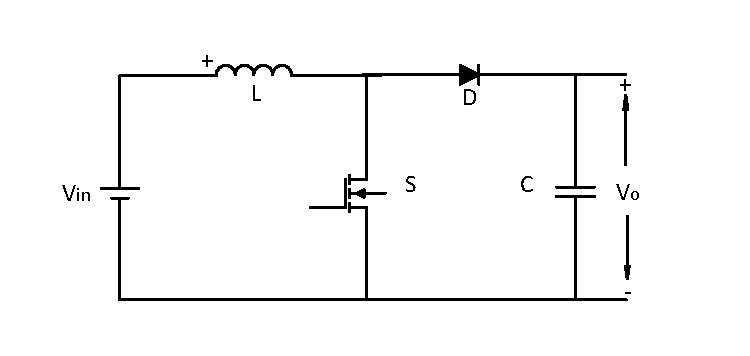
\includegraphics[width=0.8\textwidth]{figures/aConventionalBoost/ConventionalBoostConverter.pdf}
    \caption{Conventional Boost Converter}
	\label{fig:CBC}
\end{figure}

\subsection{Operation Modes}\label{sec:CBC_OP}

\subsubsection{Switch ON (Figure~\ref{fig:CBC_ON}):}

When the switch is ON,
the inductor is being charged and the capacitor discharges over the load resistor.

\begin{figure}[H]
   \centering
   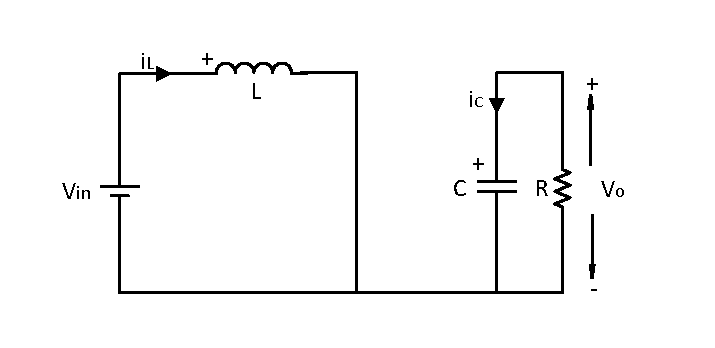
\includegraphics[width=0.8\textwidth]{figures/aConventionalBoost/ConventionalBoostConverterON.pdf}
    \caption{Conventional Boost Converter Switch ON}
	\label{fig:CBC_ON}
\end{figure}

In this case we have:
\begin{equation}
	V_L = V_{in}
	\label{eq:CBC_SWON1}
\end{equation}
where
\begin{equation}
	V_L = L \frac{di}{dt}
	\label{eq:CBC_SWON2}
\end{equation}
and
\begin{equation}
	V_C = V_R
	\label{eq:CBC_SWON3}
\end{equation}
The capacitor current discharges over the resistor:
\begin{equation}
	i_C = -\frac{V_o}{R}
	\label{eq:CBC_SWON4}
\end{equation}
\subsubsection{Switch OFF (Figure ~\ref{fig:CBC_OFF}):}

\begin{figure}[H]
   \centering
   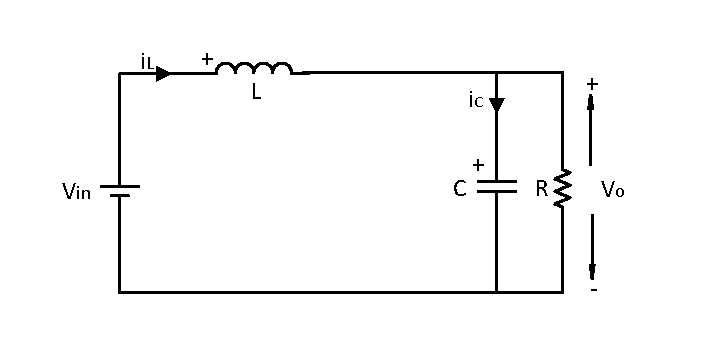
\includegraphics[width=0.8\textwidth]{figures/aConventionalBoost/ConventionalBoostConverterOFF.pdf}
    \caption{Conventional Boost Converter Switch OFF}
	\label{fig:CBC_OFF}
\end{figure}

When the switch is OFF,
the capacitor is being charged and this is the mode when the boosting happens.

In this case we have:
\begin{equation}
	V_L = V_{in} - V_o
	\label{eq:CBC_SWOFF1}
\end{equation}

\begin{equation}
	i_C = i_L -\frac{V_o}{R}
	\label{eq:CBC_SWOFF2}
\end{equation}

\begin{figure}[H]
   \centering
   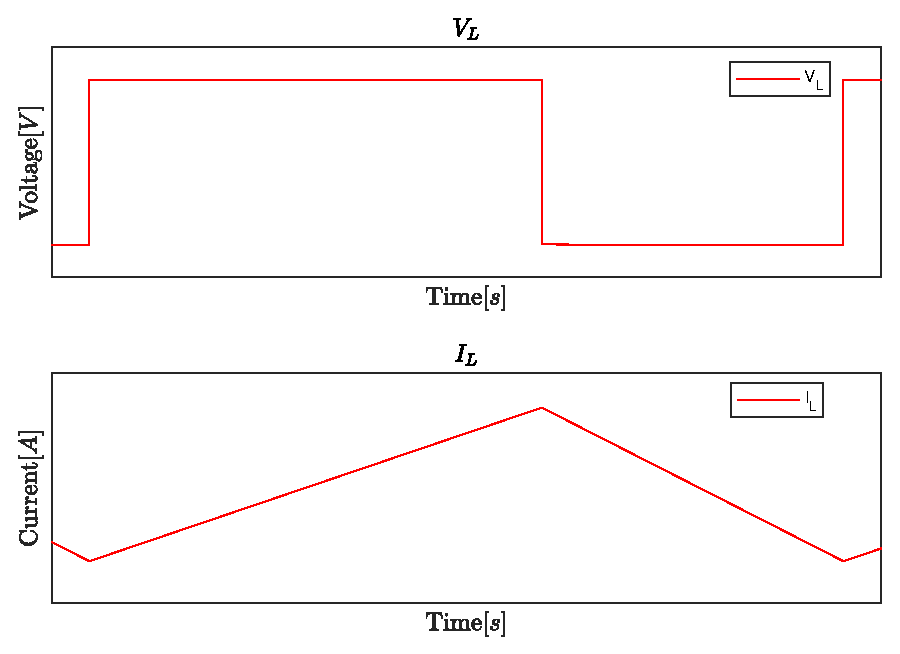
\includegraphics[width=0.8\textwidth]{figures/aConventionalBoost/LvAndLi.eps}
    \caption{CBC Inductor Wave Forms}
	\label{fig:CBC_InductorWaveForms}
\end{figure}

\subsection{Conversion ratio}\label{sec:conversionRatio}

Based on inductor volt-second balance, the conversion ratio can be calculated:

\begin{equation}
	\int_{0}^{T_s} v_L(t)dt = V_{in}D + (V_{in}-V_{out})(1-D) = 0
	\label{eq:CBC_VISB}
\end{equation}

\begin{equation}
	\frac{V_o}{V_{in}} = \frac{1}{1-D}
	\label{eq:CBC_CR}
\end{equation}

\subsection{Inductor current ripple}\label{sec:CBC_ICR}

The inductor current slope for the interval from 0 to $DT_s$ can be found as:

\begin{figure}[H]
   \centering
   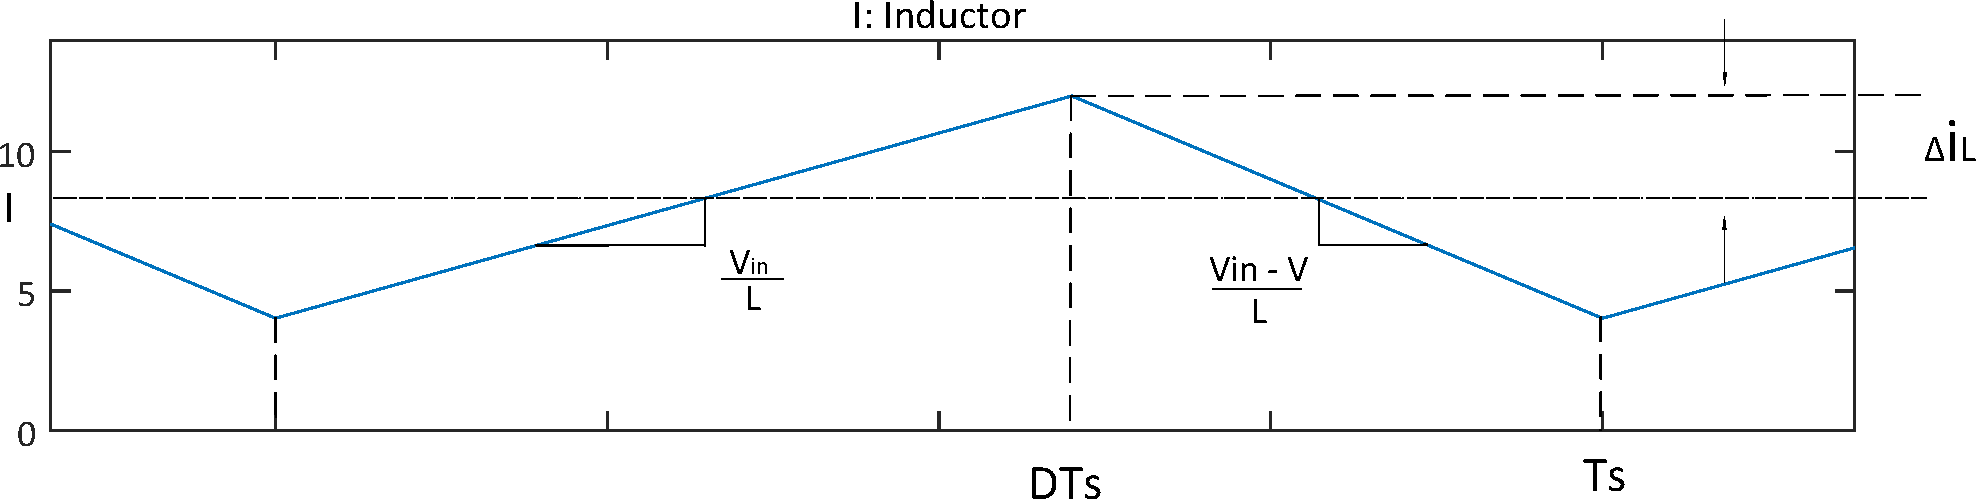
\includegraphics[width=\textwidth]{figures/aConventionalBoost/InductorCurrent.pdf}
    \caption{CBC Inductor Current Ripple}
	\label{fig:CBC_InductorCurrent}
\end{figure}


\begin{equation}
	\frac{di_L(t)}{dt} = \frac{v_L(t)}{L} = \frac{V_{in}}{L}
	\label{eq:CBC_ICR1}
\end{equation}

and the current slope for the interval (1 - DTs):

\begin{equation}
	\frac{di_L(t)}{dt} = \frac{v_L(t)}{L} = \frac{V_{in} - V}{L}
	\label{eq:CBC_ICR2}
\end{equation}

The change of inductor current during the first subinterval is:

\begin{equation}
	2\Delta i_L = \frac{V_{in}}{L}DT_s \Rightarrow
  \Delta i_L = \frac{V_{in}}{2L}DT_s
	\label{eq:CBC_ICR3}
\end{equation}

The inductor should be chosen such that a desired current ripple magnitude is optained.

\subsection{Capacitor voltage ripple}\label{sec:CBC_CVR}

\begin{figure}[H]
   \centering
   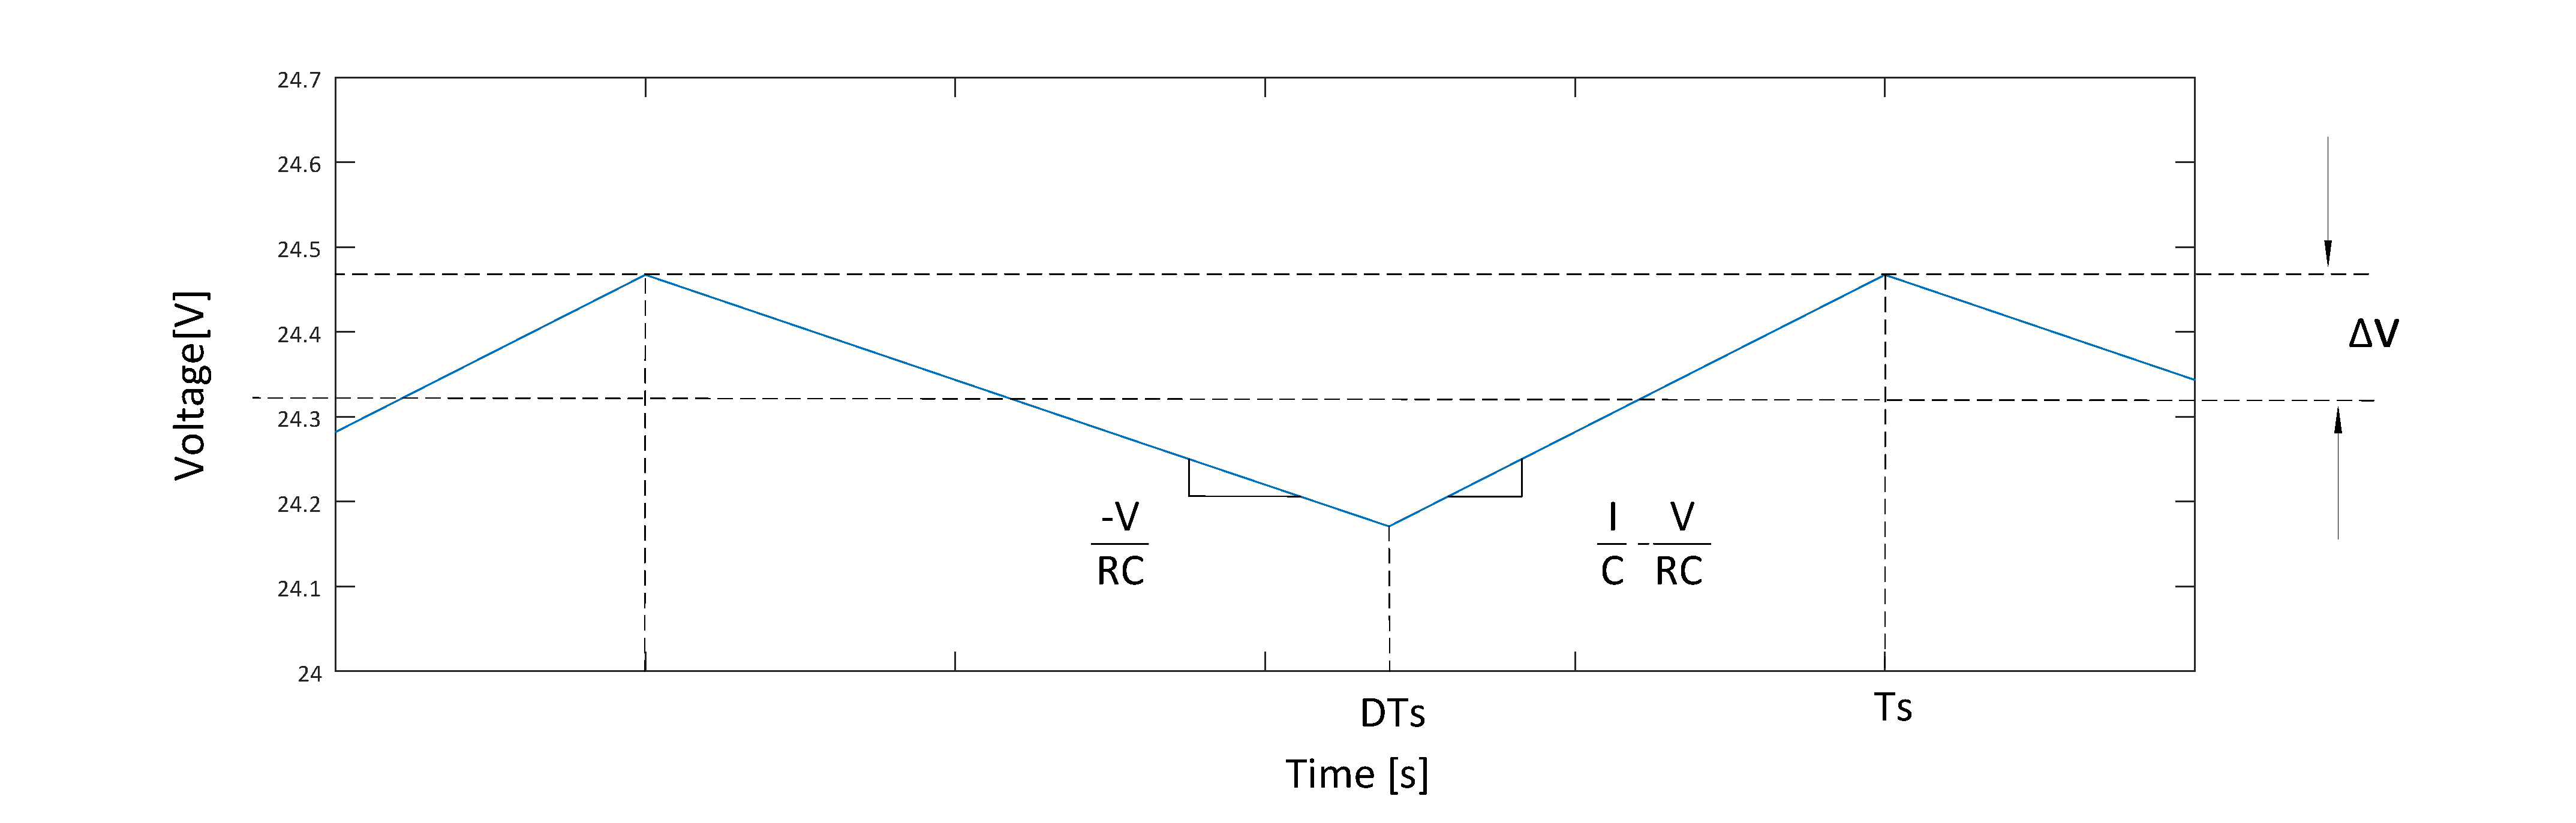
\includegraphics[width=\textwidth]{figures/aConventionalBoost/CapacitorVoltage.pdf}
    \caption{Capacitor Voltage Ripple}
	\label{fig:CBC_CVR1}
\end{figure}

The capacitor voltage slope for the interval from 0 to DTs can be found as:

\begin{equation}
	\frac{dv_c(t)}{dt} = \frac{i_c(t)}{C} = \frac{-V}{RC}
	\label{eq:CBC_CVR2}
\end{equation}

and the voltage slope for the interval (1 - DTs):

\begin{equation}
	\frac{dv_c(t)}{dt} = \frac{i_c(t)}{C} = \frac{I}{C} - \frac{V}{RC}
	\label{eq:CBC_CVR3}
\end{equation}

The change of capacitor voltage during the first subinterval is:

\begin{equation}
	-2\Delta v = \frac{-V}{RC}DT_s \Rightarrow
  \Delta v = \frac{V}{2RC}DT_s
	\label{eq:CBC_CVR4}
\end{equation}

The capacitor should be chosen according to the desired voltage ripple.

\subsection{Design Example}\label{sec:CBC_DE}

If we consider a design for a boost converter that will have an output of 25V from a 10V source, with a continuous inductor current and an output voltage of less than one percent, we will have the following parameters:\\
V\textsubscript{in} = 10 V, V\textsubscript{out} = 25 V and D = 0.6. Also,
a load resistor of 40 $\Omega$ and a  switching frequency of 25kHz are considered for the design.


By the fact that the average power supplied by the source must be the same as the average power absorbed by the load resistor, the output power can be obtained by:

\begin{equation}
	P_o = \frac{V^2_o}{R} = V_oI_o
	\label{eq:CBC_CVR4}
\end{equation}

and the input power is $V_{in}I_s = V_{in}I_L$

\begin{equation}
	\Rightarrow V_{in}I_L = \frac{V^2_o}{R} = \frac{[V_{in}/(1-D)]^2}{R}
	\label{eq:CBC_CVR4}
\end{equation}

solving for I\textsubscript{L}, we get:

\begin{equation}
	I_L = \frac{V_{in}}{(1-D)^2R}
	\label{eq:CBC_CVR4}
\end{equation}

The maximum and minimum inductor current can be determined by:

\begin{equation}
	I_{max} = I_L + \Delta i_L = \frac{V_{in}}{(1-D)^2R} + \frac{V_{in}DT_s}{2L}
	\label{eq:CBC_CVR4}
\end{equation}

\begin{equation}
	I_{min} = I_L - \Delta i_L = \frac{V_{in}}{(1-D)^2R} - \frac{V_{in}DT_s}{2L}
	\label{eq:CBC_CVR4}
\end{equation}


The induction current has to be continuous, so it has to be always positive. This means that I\textsubscript{L} has to be positive and the boundary between continuous and discontinuous inductor current is determined from:\\
\begin{equation}
	I_{min} = 0 = \frac{V_{in}}{(1-D)^2R} - \frac{V_{in}DT_s}{2L}
\end{equation}

\begin{equation}
	\frac{V_{in}}{(1-D)^2R} = \frac{V_{in}DT_s}{2L} = \frac{V_{in}D}{2Lf}
\end{equation}


So, the minimum combination of inductance and switching frequency for continuous current is:

\begin{equation}
L_{min} = \frac{D(1-D)^2R}{2f} = \frac{0.6(1-0.6)^2 40}{2\cdot25000} = 76.8\mu F
\end{equation}


L = 120 $\mu$F is selected to provide a margin to ensure continuous current.
Then, using Equation~\ref{eq:CBC_CVR4}, we can find the average inductor current.

\begin{equation}
I_L = \frac{V_{in}}{(1-D)^2R} = \frac{10}{(1-0.6)^2(40)} = 1.56 A
\end{equation}\\
Afterwards, the current ripple according to Figure~\ref{fig:CBC_InductorCurrent} is calculated using Equation~\ref{eq:CBC_CVR3}

\begin{equation}
\Delta i_L = \frac{V_{in}DT}{2L} = \frac{10\cdot 0.6}{2\cdot 100\cdot 10^{-6}\cdot 25000} = 1 A
\end{equation}\\
$I_{max} = 1.56 + 1 = 2.56 A$ , 
$I_{min} = 1.56 - 1 = 0.56 A$


Based on equation ~\ref{eq:CBC_CVR4}, the minimum capacitance required to limit the output voltage ripple to 1 percent is:

\begin{equation}
C_{min} = \frac{D}{R(\Delta V_o/V)f} = \frac{0.6}{40\cdot 0.01\cdot 25000 } = 60\mu F
\end{equation}\\
A capacitor of 80 $\mu$ F was chosen to provide a satisfactory margin.\\

To confirm the calculations, the circuit was built in SIMULINK, using the calculated parameters presented on Table~\ref{tab:CBC}.

\begin{table}[H]
\begin{center}
\caption {Simulation parameters for CBC} \label{tab:CBC} 
\begin{tabular}{|l|l|}
\cline{1-2}
\textbf{Parameter} & \textbf{Value}  \\ \cline{1-2}
Input Voltage $V_{in}$          &      10V   \\ \cline{1-2}
Load(R)   & 40$\Omega$           \\ \cline{1-2}
Capacitance(C)          &       80$\mu$F     \\ \cline{1-2}
Inductance(L)          &      120$\mu$F      \\ \cline{1-2}
Duty cycle(D)          &     0.6       \\ \cline{1-2}
Switching Frequency($f$)          &      25kHz      \\ \cline{1-2}
\end{tabular}
\end{center}
\end{table}

The simulation presented on Figure~\ref{fig:CBC_Sim} is using an ideal switch for the active device.

\begin{figure}[H]
   \centering
   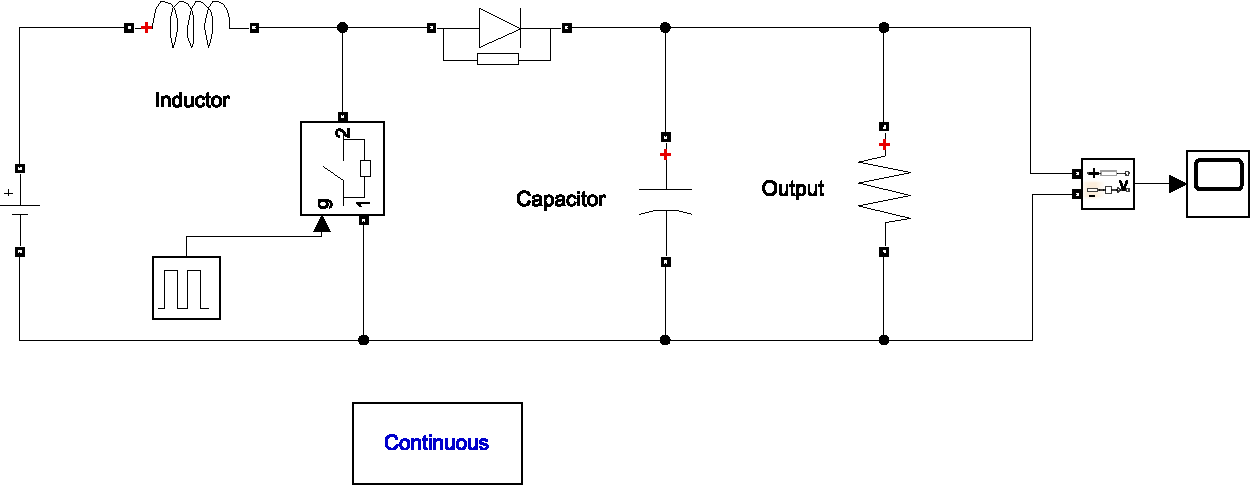
\includegraphics[width=0.8\textwidth]{figures/aConventionalBoost/CBCpic.pdf}
    \caption{Conventional Boost Converter}
	\label{fig:CBC_Sim}
\end{figure}

The results from the simulation are presented on Figure~\ref{fig:CBC_SimResults} and it can be observed that they match with the calculations. 

\begin{figure}[H]%
    \centering
    %\subfloat[Switch ON\label{SI_ON}]
    {{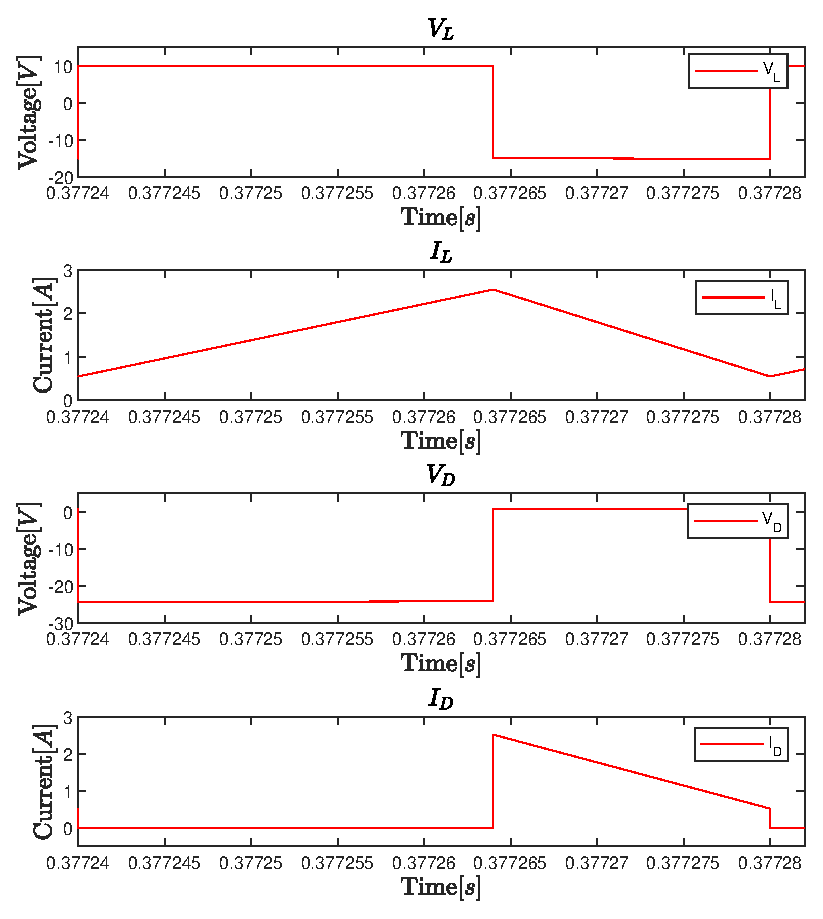
\includegraphics[width=0.8\textwidth]{figures/aConventionalBoost/CBC_V_LtoI_D.eps} }}%
    \qquad
    \subfloat{{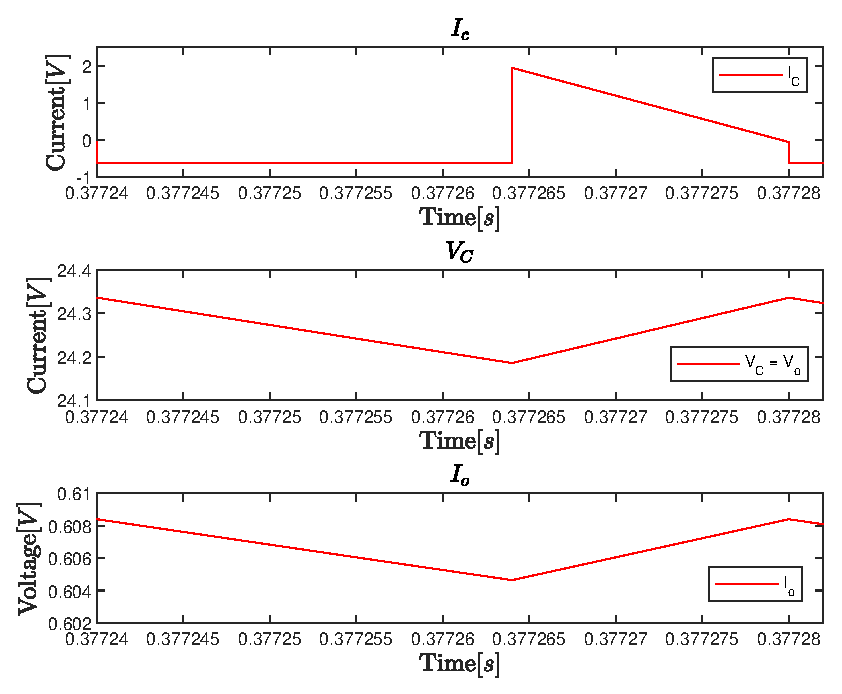
\includegraphics[width=0.8\textwidth]{figures/aConventionalBoost/CBC_I_CtoI_out.eps} }}%  
    \caption{Simulation results}%
     \label{fig:CBC_SimResults}% 
\end{figure}

\section{Switched Inductor}\label{ch:SIBC}
The Switched Inductor Boost Converter (SIBC) is a small alternation to the Conventional Boost Converter mentioned in Chapter \ref{ch:CBC}.
It only adds passive components to an already known topology,
which means the same switching scheme can be used.
\subsection{Additions from Conventional BC}
In the SIBC,
the single inductor from the Conventional BC gets replaced by two inductors and three diodes,
connected as shown in Figure \ref{fig:SwitchedInductor}.

\begin{figure}
   \centering
   \includegraphics[width=\textwidth]{figures/bSwitchedInductor/switched_inductor.pdf}
    \caption{Switched inductor boost converter circuit}
	\label{fig:SwitchedInductor}
\end{figure}


With this configuration,
the inductors form two different topologies during the ON and OFF states. By reversing the biasing of the diodes the inductors are connected in parallel during ON state and series during OFF state.  \todo[color=c04b]{refer to figure maybe} 


\subsection{Switching States}
The same switching scheme as for the Conventional BC can be used,
as mentioned earlier.
The equivalent circuits during the on and off stage are shown in Figure \ref{fig:SI_States}.

\begin{figure}[H]%
    \centering
    \subfloat[Switch ON\label{SI_ON}]
    {{\includegraphics[width=6.5cm]{figures/bSwitchedInductor/switched_inductorON.pdf} }}%
    \qquad
    \subfloat[Switch OFF\label{SI_OFF}]{{\includegraphics[width=6.5cm]{figures/bSwitchedInductor/switched_inductorOFF.pdf} }}%  
    \caption{Switching states of the SIBC}%
     \label{fig:SI_States}% 
\end{figure}

\subsubsection{ON State}
While the switch is ON, diodes D\textsubscript{1} and D\textsubscript{2} are forward biased and diode ? is reverse biased.
This constructs a parallel conection between the inductors, as seen in Figure \ref{SI_ON}.
\\*
In this case, we can use KVL to build the eqation: 

\begin{equation}
	V_L=V_{in}
	\label{eq:SI_KVL_ON}
\end{equation}

\subsubsection{OFF State}
While the switch is OFF, the complete opposite happens, where only D\textsubscript{2} remains forward biased and forms a series connections between the inductors (shown on Figure \ref{SI_OFF}).
In a configuration like this we can assume equal split of the pottential across the inductors and using KVL construct the equation:
\begin{equation}
	V_{in}-2V_L-V_o=0
	\label{eq:SI_KVL_OFF}
\end{equation}
Subsequetially reformed as:
\begin{equation}
	V_L=\frac{V_{in} - V_o}{2}
	\label{eq:SI_KVL_OFF2}
\end{equation}
 \\*
Reforming the Inductor voltage-second balance(Explained in Sections \ref{sec:convertionRatio} for the current topology, we get the following relationship:

\begin{equation}
	V_{L(ON)}D+V_{L(OFF)}(1-D)=0
	\label{eq:SI_IVSB}
\end{equation}
Substituting the already derived expressions for V\textsubscript{L}:
\begin{equation}
	V_{in}D+\frac{V_{in} - V_o}{2}(1-D)=0
	\label{eq:SI_IVSB2}
\end{equation}
Subsequenlty the input/output relationship can be stated as:

\begin{equation}
	\frac{V_o}{V_{in}} = \frac{1+D}{1-D}
	\label{eq:pumpHeadMode5}
\end{equation}


\subsection{Single Switch Quadratic BC}\label{ch:SSQBC}
\todo[color=c04c,inline]{testing the colors}
\section{Conventional Three Level Boost Converter}\label{ch:TLBC}

The conventional three level boost converter is the first variation of the conventional BC that includes not only passive components, but also an additional active component. This, as in all other topologies discussed, increases the ratio between output and input, this time in a completely linear manner, as it will be proven in the this section. 

\subsection{Additions from Conventional BC}
In the CTLBC, a second switch is included, together with another capacitor to go in parallel with it, An additional diode is included to allow both switches to conduct at the same time without causing damage to the circuit.The full schematic can be seen on Fig. \ref{fig:CTLBC}  

\begin{figure} [H]
   \centering
   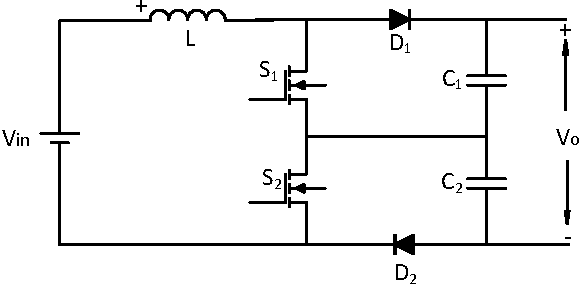
\includegraphics[width=0.6\textwidth]{figures/dConventionalThreeLevelBC/Three_level.pdf}
    \caption{Conventional Three Level Boost Converter circuit}
	\label{fig:CTLBC}
\end{figure}
\subsection{Switching States}
As there are two switches in this topology, a different switching pattern is required in comparison to the Conventional BC. The pattern of choice is shifting the signal to the second switch by The angle is 90$^\circ$ degrees.
In this case, there are four possible states, corresponding to all possible combinations between the switches. Not all of them occur for one given duty cycle value. 
The equivalent circuits during the on and off stages are shown in Figure \ref{fig:CTLBC_States}. Here again we assume the capacitors are the same size and that the duty ratio applied to the two switches is the same. 
\vspace{-5mm}
\begin{figure}[H]%
    \centering
    \subfloat[Switch S\textsubscript{1} ON, Switch S\textsubscript{2} ON\label{CTLBC_ONON}]
    {{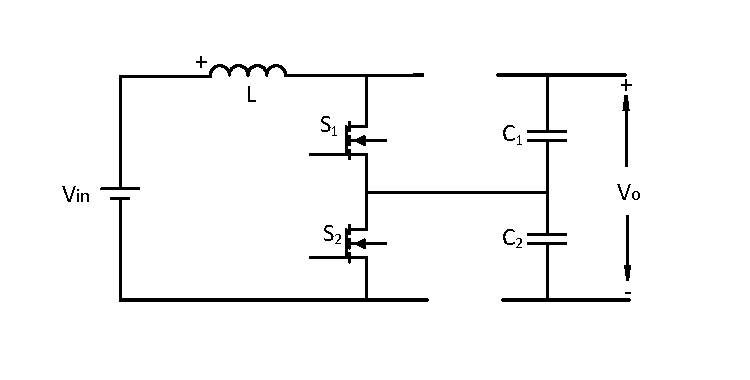
\includegraphics[width=0.45\textwidth]{figures/dConventionalThreeLevelBC/Three_levelONON.pdf} }}%
    \qquad
    \subfloat[Switch S\textsubscript{1} ON, Switch S\textsubscript{2} OFF\label{CTLBC_ONOFF}]{{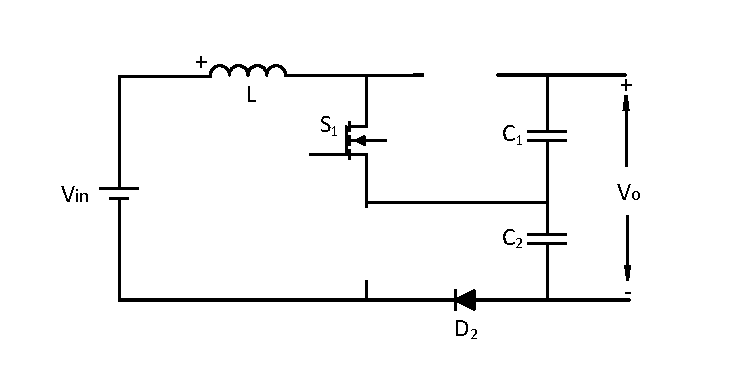
\includegraphics[width=0.45\textwidth]{figures/dConventionalThreeLevelBC/Three_levelONOFF.pdf} }}%  
   \qquad
        \subfloat[Switch S\textsubscript{1} OFF, Switch S\textsubscript{2} ON\label{CTLBC_OFFON}]
    {{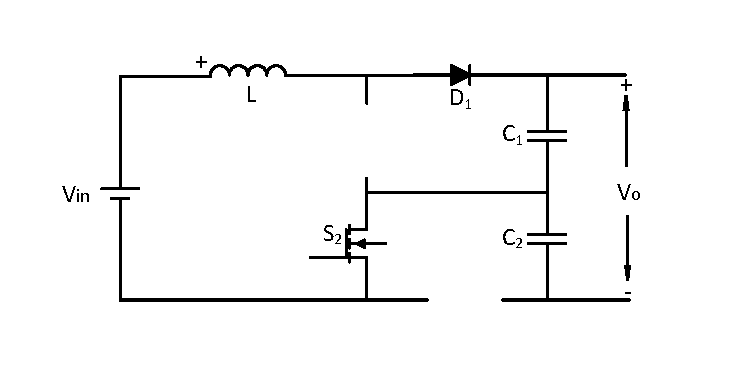
\includegraphics[width=0.45\textwidth]{figures/dConventionalThreeLevelBC/Three_levelOFFON.pdf} }}%
    \qquad
    \subfloat[Switch S\textsubscript{1} OFF, Switch S\textsubscript{2} OFF\label{CTLBC_OFFOFF}]{{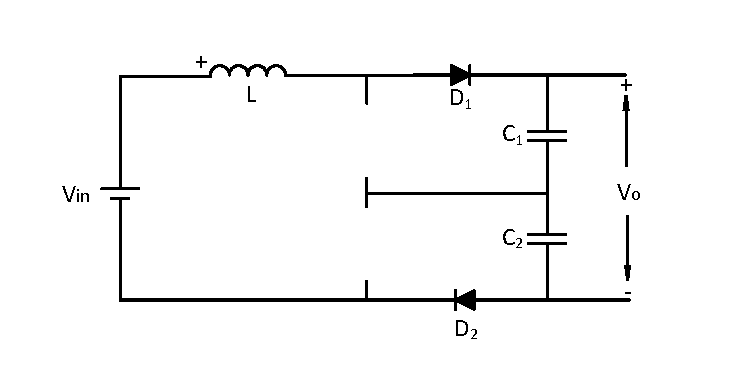
\includegraphics[width=0.45\textwidth]{figures/dConventionalThreeLevelBC/Three_levelOFFOFF.pdf} }}%  
    \caption{Switching states of the SIBC}%
     \label{fig:CTLBC_States}% 
     
\end{figure}
\subsubsection{Switch S\textsubscript{1} ON, Switch S\textsubscript{2} ON State}
Here we have got a replica of the ON state of a conventional boost converter, as both switches conduct and both diodes are reverse biased.(Can be seen on Figure \ref{CTLBC_ONON}) A loop is formed with the inductor and the power supply. We use KVL to express the voltage over the inductor as: 

\begin{equation}
	V_{L}=V_{in}
	\label{eq:CTLBC_KVL_ONON}
\end{equation}
Another loop is formed with the two capacitor and the output.This loop can be observed over all the rest of the states as well. Again assuming the capacitors are the same size, the voltage would split equally across them and the loop can be expressed via KVL as: 

\begin{equation}
	V_O=2V_C
	\label{eq:CTLBC_KVL_ONON2}
\end{equation}


\subsubsection{Switch S\textsubscript{1} ON, Switch S\textsubscript{2} OFF State}
While only switch S\textsubscript{1}conducts, diode D\textsubscript{2} is forwards biased and extends the loop over C\textsubscript{2}.(Can be seen on Figure \ref{CTLBC_ONOFF}) We use KVL to express the voltage over the inductor as: 
\begin{equation}
	V_{L}=V_{in}-V_C
	\label{eq:CTLBC_KVL_ONOFF}
\end{equation}
 
\subsubsection{Switch S\textsubscript{1} OFF, Switch S\textsubscript{2} ON State}
Similar to the previous state, S\textsubscript{2}conducts, diode D\textsubscript{1} is forwards biased and extends the loop over C\textsubscript{1} (Can be seen on Figure \ref{CTLBC_OFFON}). As already stated, capacitor sizes and duty cycles are assumed equal, therefore no change in KVL between the two loops: 
\begin{equation}
	V_{L}=V_{in}-V_C
	\label{eq:CTLBC_KVL_OFFON}
\end{equation}

\subsubsection{Switch S\textsubscript{1} OFF, Switch S\textsubscript{2} OFF State}
With both switches open the circuit formed is equivalent to the OFF state in a conventional BC.(Can be seen on Figure \ref{CTLBC_OFFOFF}) We use KVL to express the voltage over the inductor as: 
\begin{equation}
	V_{L}=V_{in}-V_{O}
	\label{eq:CTLBC_KVL_OFFOFF}
\end{equation}

To find an expression for the output-input gain of the topology, we refer back to the IVSB (Sec. \ref{sec:convertionRatio})and formulate the expression that is valid for both switches since Eq. \ref{eq:CTLBC_KVL_ONOFF} and Eq.\ref{eq:CTLBC_KVL_OFFON} are identical:
\begin{equation}
	V_{L(ON)}D+V_{L(OFF)}(1-D)=0
	\label{eq:CTLBC_IVSB}
\end{equation}
Substituting the already derived expressions for V\textsubscript{L}:

\begin{equation}
	V_{in}D+(V_{in} - V_C)(1-D)=0
	\label{eq:CTLBC_IVSB2}
\end{equation}
Reforming this equation we get: 
\begin{equation}
	V_{in}=V_C(1-D)
	\label{eq:CTLBC_IVSB3}
\end{equation}
Using the already derived expression for V\textsubscript{O} in Eq.\ref{eq:CTLBC_KVL_ONON2} we can directly form the output-input function: 
\begin{equation}
	\frac{V_O}{V_{in}}=\frac{2}{(1-D)}
	\label{eq:CTLBC_IVSB4}
\end{equation}
Otherwise expressed, the gain of the CTLBC is twice the one of a conventional BC. 
\todo[color=c04,inline]{Add simulation results}
\chapter{Switched Inductor}\label{ch:SIBC}
The Switched Inductor Boost Converter (SIBC) is a small alternation to the Conventional Boost Converter mentioned in Chapter \ref{ch:CBC}.
It only adds passive components to an already known topology,
which means the same switching scheme can be used.
\section{Additions from Conventional BC}
In the SIBC,
the single inductor from the Conventional BC gets replaced by two inductors and three diodes,
connected as shown in Figure \ref{fig:SI}.

\missingfigure{switched Inductor} \label{fig:SI}

With this configuration,
both inductors get charged up during the on stage
and can discharge into the output capacitor during the off stage.
The diodes prevent the current to run back into the DC link \todo[color=c02]{maybe rewrite this}
thus preventing damage.


\section{Switching States}
The same switching scheme as for the Conventional BC can be used,
as mentioned earlier.
The equivalent circuits during the on and off stage are shown in Figure \ref{fig:OnOffSIBC}.

\missingfigure{On and off stage equivalents of the SIBC}\label{fig:OnOffSIBC}

some text
\todo[color=c02,inline]{calculations}
some text
\todo[color=c02,inline]{simulations}
some text

As you can see in Chapter \ref{ch:dataAcq}

If you want to write a paragraph on something,
this will still be the same line.
I will make this paragraph a little bittle longer,
so that it actually uses more than one line.
I think it does now.

New paragraphs start with a proceeding empty line in the editor.
\chapter{Bootstrap Capacitor and Boost Inductor BC}\label{ch:BCBIBC}

\chapter{PCB Design}\label{ch:PCB}

To be able to test the proposed topology,
a Printed Circuit Board (PCB) was made.

\missingfigure{some pcb design}

- 
- guidance from Sagar Mahajan \todo{reference him?}.




\printbibliography[heading=bibintoc]
\label{bib:mybiblio}
\appendix
%\chapter{System Overview}
\label{app:overview}
\begin{figure}[H]
    \centering
    \includegraphics[width=\textwidth, height=0.8\textheight, keepaspectratio]{figures/appendix/P4setup.pdf}
    \caption{Schematic Overview of the System}
	\label{fig:overview}
\end{figure}
%\chapter{Modelling}
\label{app:modelling}
\newpage
\begin{figure}[H]
	\centering
	\includegraphics[width=1\textheight, height = 1\textwidth, keepaspectratio, angle = 270]{figures/05mathematicalModelling/flowVsPressureRun34.eps}
	\caption{Data Points for Flow vs. Pressure}
\end{figure}

\begin{figure}[H]
	\centering
	\includegraphics[width=1\textheight, height = 1\textwidth, keepaspectratio,  angle = 270]{figures/05mathematicalModelling/flowVsPowerRun34.eps}
	\caption{Data Points for Flow vs. Power Consumption}
\end{figure}

\begin{figure}[H]
	\centering
	\includegraphics[width=1\textheight, height = 1\textwidth, keepaspectratio,  angle = 270]{figures/06ModelValidation/modeledStepResponse.eps}
	\caption{Modeled Step Response}
\end{figure}

%\chapter{Model Validation}
\label{app:modelValidation}
\newpage
\begin{figure}[H]
	\centering
	\includegraphics[width=1\textheight, height = 1\textwidth, keepaspectratio, angle = 270]{figures/06ModelValidation/flowVsModeledPowerConsumption.eps}
	\caption{Flow Vs. Modeled Power Consumption}
\end{figure}

\begin{figure}[H]
	\centering
	\includegraphics[width=1\textheight, height = 1\textwidth, keepaspectratio, angle = 270]{figures/06ModelValidation/flowVsModeledPressure.eps}
	\caption{Flow Vs. Modeled Pressure}
\end{figure}

\begin{figure}[H]
	\centering
	\includegraphics[width=1\textheight, height = 1\textwidth, keepaspectratio, angle = 270]{figures/06ModelValidation/modelPI.eps}
	\caption{Modeled PI Controller}
\end{figure}

\begin{figure}[H]
	\centering
	\includegraphics[width=1\textheight, height = 1\textwidth, keepaspectratio, angle = 270]{figures/06ModelValidation/modelPID.eps}
	\caption{Modeled PID Controller}
\end{figure}
%\chapter{Measured Data}
\label{app:gatheredData}
\newpage
\begin{figure}[H]
	\centering
	\includegraphics[height=\textwidth, width=\textheight, keepaspectratio, angle=270]{figures/05mathematicalModelling/measuredFlow.eps}
	\caption{Measured Flow}
\end{figure}

\begin{figure}[H]
	\centering
	\includegraphics[height=\textwidth, width=\textheight, keepaspectratio, angle=270]{figures/05mathematicalModelling/measuredPower.eps}
	\caption{Measured Power}
\end{figure}

\begin{figure}[H]
	\centering
	\includegraphics[height=\textwidth, width=\textheight, keepaspectratio, angle=270]{figures/05mathematicalModelling/measuredPressure.eps}
	\caption{Measured Pressure}
\end{figure}

\begin{figure}[H]
	\centering
	\includegraphics[height=\textwidth, width=\textheight, keepaspectratio, angle=270]{figures/04ExperimentsAndLabWork/testrun.eps}
	\caption{$Q$, $H$, $P$ and stair input $\omega P_{2in}$ at $CV_1 = 70\%$}
\end{figure}
\end{document}
